\section{REZULTATI}

\subsection{SIMULACIJE}
Skupno smo izvedli 6000 simulacij. Tri tisoč simulacij smo izvedli na način, da smo individualno spremenljivko izračunali s pomočjo simuliranih vrednosti standardnega odklona (normalna porazdelitev). S pomočjo programa MARK smo uspešno ocenili parametre v 2916 simulacijah.
Enako število simulacij smo izvedli za primer, kjer smo krivuljo za izračun individualne spremenljivke ocenili iz podatkov (empirična porazdelitev). Pri oceni parametrov smo bili uspešni 2681-krat (Preglednica \ref{tab:tabela1}).

Da parametrov nekaterih simulacij nismo uspešno ocenili, je po pričakovanjih. Zaradi določene strukture podatkov je možno, da optimizacijski kriterij znotraj parametrskega prostora ne najde optimuma ali pa so ocenjeni parametri na intervalu $- \infty < x < \infty$. Tiste simulacije, ki niso dale smiselnega rezultata, smo iz analize izključili.

Na polno obremenjenem računalniku je bila simulacija izračuna individualne spremenljivke končana v približno 48 urah. Nadaljnje analize lova-ponovnega ulova ter priprava podatkov za analizo pa so zahtevale še dodatnih šest ur.

Zaznati je mogoče vzorec v številu uspešnih simulacij glede na uporabljeno funkcijo. Število uspešnih simulacij glede na število generiranih osebkov in število odlovnih intervalov se med skupinama razlikuje. Večina neuspelih simulacij pri uporabi empirične funkcije je za najmanjše število odlovnih intervalov ($K=5$).


\begin{table}[!htb]
  \caption[Preglednica števila simulacij, ki so dale smiseln rezultat]{Preglednica števila simulacij, ki so dale smiseln rezultat. Prikaz števila simulacij, kjer smo uspešno ocenili parametre, glede na funkcijo, ki je bila uporabljena za izračun individualne spremenljivke. V vrsticah je povprečno število generiranih osebkov znotraj območja vzorčenja ($N$), v stolpcih pa število odlovnih intervalov ($K$). Uspešno izračunanih simulacij z empirično funkcijo je nekoliko manj. Za lažjo predstavo v spodnji matriki prikazujemo razliko med zgornjima preglednicama tako, da smo empirični (levo) odšteli normalno (desno) preglednico. Pretežni delež neuspelih simulacij je predvsem na račun simulacij, ki imajo 5 odlovnih intervalov in/ali manjše število simuliranih osebkov (nižja gostota).

  \medskip

  Table \ref{tab:tabela1}: Number of simulations for which model parameters have been produced based on function used to calculate individual covariate. Rows represent average number of individuals generated within the sampling polygon ($N$), columns represent number of sampling sessions ($K$). For the empirical function (left), number of successfully estimated simulations is slightly lower. Simulations with lower numbers of sampling sessions and simulated individuals were less likely to produce model estimates. Table on the right shows difference between left and center table.
}
  \label{tab:tabela1}
\begin{tabular}{cc}
    \begin{minipage}{.33\linewidth}
      \caption*{Empirična funkcija}
      \resizebox{\columnwidth}{!}{%
        \begin{tabular}{rccc}
          \toprule
           & \textbf{$K=5$} & \textbf{$k=10$} & \textbf{$K=15$} \\
          \midrule
          $N=20$ & 142 & 187 & 190 \\
          $N=30$ & 141 & 192 & 178 \\
          $N=40$ & 135 & 182 & 185 \\
          $N=50$ & 168 & 212 & 194 \\
          $N=60$ & 171 & 186 & 218 \\
          \bottomrule
        \end{tabular}
        }
    \end{minipage}%

    \begin{minipage}{.33\linewidth}
      \caption*{Normalna funkcija}
      \resizebox{\columnwidth}{!}{%
        \begin{tabular}{rccc}
          \toprule
           & \textbf{$K=5$} & \textbf{$k=10$} & \textbf{$K=15$} \\
          \midrule
          $N=20$ & 188 & 209 & 197 \\
          $N=30$ & 179 & 205 & 183 \\
          $N=40$ & 175 & 190 & 185 \\
          $N=50$ & 191 & 212 & 195 \\
          $N=60$ & 199 & 190 & 218 \\
          \bottomrule
        \end{tabular}
        }
    \end{minipage}%

    \begin{minipage}{.33\linewidth}
      \caption*{Razlike med matrikama}
      \resizebox{\columnwidth}{!}{%
        \begin{tabular}{rccc}
          \toprule
           & \textbf{$K=5$} & \textbf{$k=10$} & \textbf{$K=15$} \\
          \midrule
          $N=20$ & -46 & -22 & -7 \\
          $N=30$ & -38 & -13 & -5 \\
          $N=40$ & -40 & -8 & 0 \\
          $N=50$ & -23 & 0 & -1 \\
          $N=60$ & -28 & -4 & 0 \\
          \bottomrule
        \end{tabular}
        }
    \end{minipage}
\end{tabular}
\end{table}

\subsection{PARAMETER P MODELOV $M_0$ IN $M_{sp}$ PO HUGGINSU}
Za modela $M_0$ in $M_{sp}$ smo predpostavili, da sta parametra $p$ in $c$ enaka. Ulovljivost v prvem in vseh ostalih odlovnih intervalih predpostavljamo enako. Zato v analizi obravnavamo le parameter ulovljivosti $p$. Za lažjo primerjavo smo izračunali razmerje med ocenjeno in simulirano vrednostjo $p$ (slika \ref{sli:slika3}). Model TIRM oceni $p$ za dve skupini, kar ni neposredno primerljivo s parametrom p po Hugginsovem modelu, zato tega nismo podrobneje preučili.

V povprečju je ulovljivost za vse simulacije in modele podcenjena in je približno med 0.35 in 0.4 deleža simulirane vrednosti. Ulovljivost, ocenjena po modelu $M_{sp}$, je nekoliko bolj podcenjena ne glede na to, s pomočjo katere porazdelitve izračunamo individualno spremenljivko. V povprečju je ulovljivost za primer empirične porazdelitve za oba modela nekoliko nižja (za približno 0.01). Vidimo tudi, da se razlika med modeloma rahlo zmanjša s povečanjem simulirane ulovljivosti (slika \ref{sli:slika3}).

\subsubsection[\bfseries Primerjava simulirane in ocenjene ulovljivosti glede na porazdelitev]{Primerjava simulirane in ocenjene ulovljivosti glede na porazdelitev}
\subsubsubsection{Empirična porazdelitev}
Povprečje deleža simulirane vrednosti preprostega $M_0$ modela je 0.397, modela z individualno spremenljivko $M_{sp}$ pa za 0.035 nižja.

\begin{verbatim}
Call:
glm(formula = p.val ~ p.var, data = xep)

Deviance Residuals:
 	Min    	1Q	Median    	3Q   	Max
-0.36868  -0.16667  -0.07254   0.09971   1.44373

Coefficients:
              	Estimate Std. Error t value Pr(>|t|)
(Intercept)   	0.397081   0.001467  270.69   <2e-16 ***
p.varp.target.sp -0.035010   0.002075  -16.88   <2e-16 ***
---
Signif. codes:  0 ‘***’ 0.001 ‘**’ 0.01 ‘*’ 0.05 ‘.’ 0.1 ‘ ’ 1

(Dispersion parameter for gaussian family taken to be 0.05769313)

	Null deviance: 3109.8  on 53619  degrees of freedom
Residual deviance: 3093.4  on 53618  degrees of freedom
AIC: -786.36
\end{verbatim}

\subsubsubsection{Normalna porazdelitev}
Povprečje deleža simulirane vrednosti preprostega $M_0$ modela je 0.387, modela z individualno spremenljivko $M_{sp}$ pa 0.349 (0.038 nižja).

\begin{verbatim}
Call:
glm(formula = p.val ~ p.var, data = xep)

Deviance Residuals:
 	Min    	1Q	Median    	3Q   	Max
-0.35876  -0.16239  -0.07163   0.09433   1.45364

Coefficients:
              	Estimate Std. Error t value Pr(>|t|)
(Intercept)   	0.387167   0.001381  280.29   <2e-16 ***
p.varp.target.sp -0.037886   0.001953  -19.39   <2e-16 ***
---
Signif. codes:  0 ‘***’ 0.001 ‘**’ 0.01 ‘*’ 0.05 ‘.’ 0.1 ‘ ’ 1

(Dispersion parameter for gaussian family taken to be 0.05563641)

	Null deviance: 3265.5  on 58319  degrees of freedom
Residual deviance: 3244.6  on 58318  degrees of freedom
AIC: -2972.7
\end{verbatim}

\begin{figure}[H]
\centering
\begin{subfigure}[b]{0.75\textwidth}
  \centering
  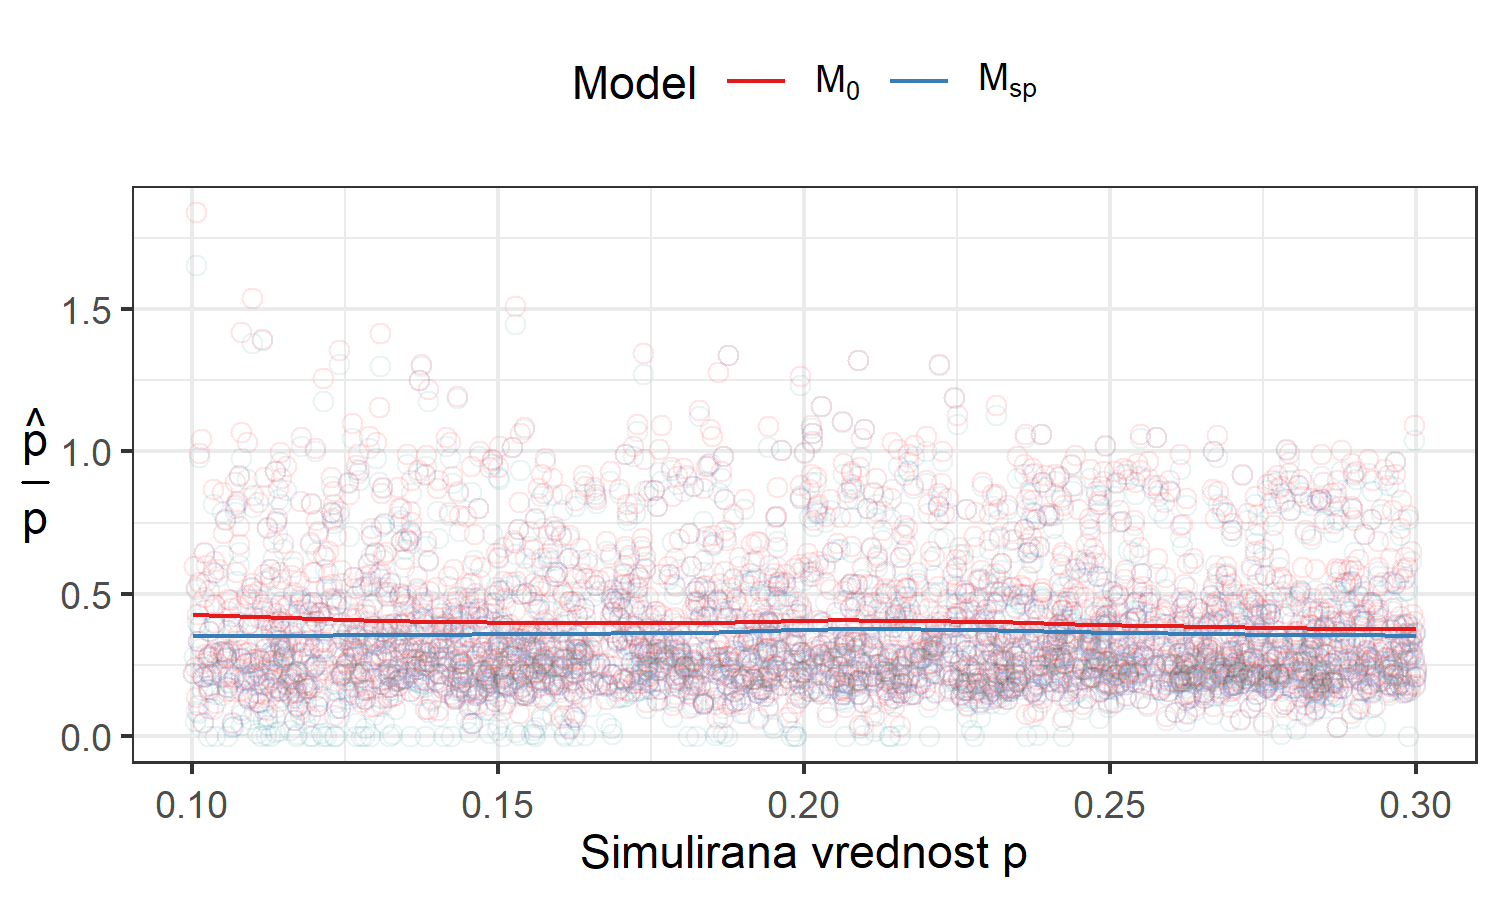
\includegraphics[width=1\linewidth]{C:/Users/romunov/Documents/workspace/doktorat/analiza/figures/E-0a_pristranskost_1_in_sp_ocene_ulovljivosti.png}
  \label{sli:sub3.1}
\end{subfigure}

\begin{subfigure}[b]{0.75\textwidth}
  \centering
  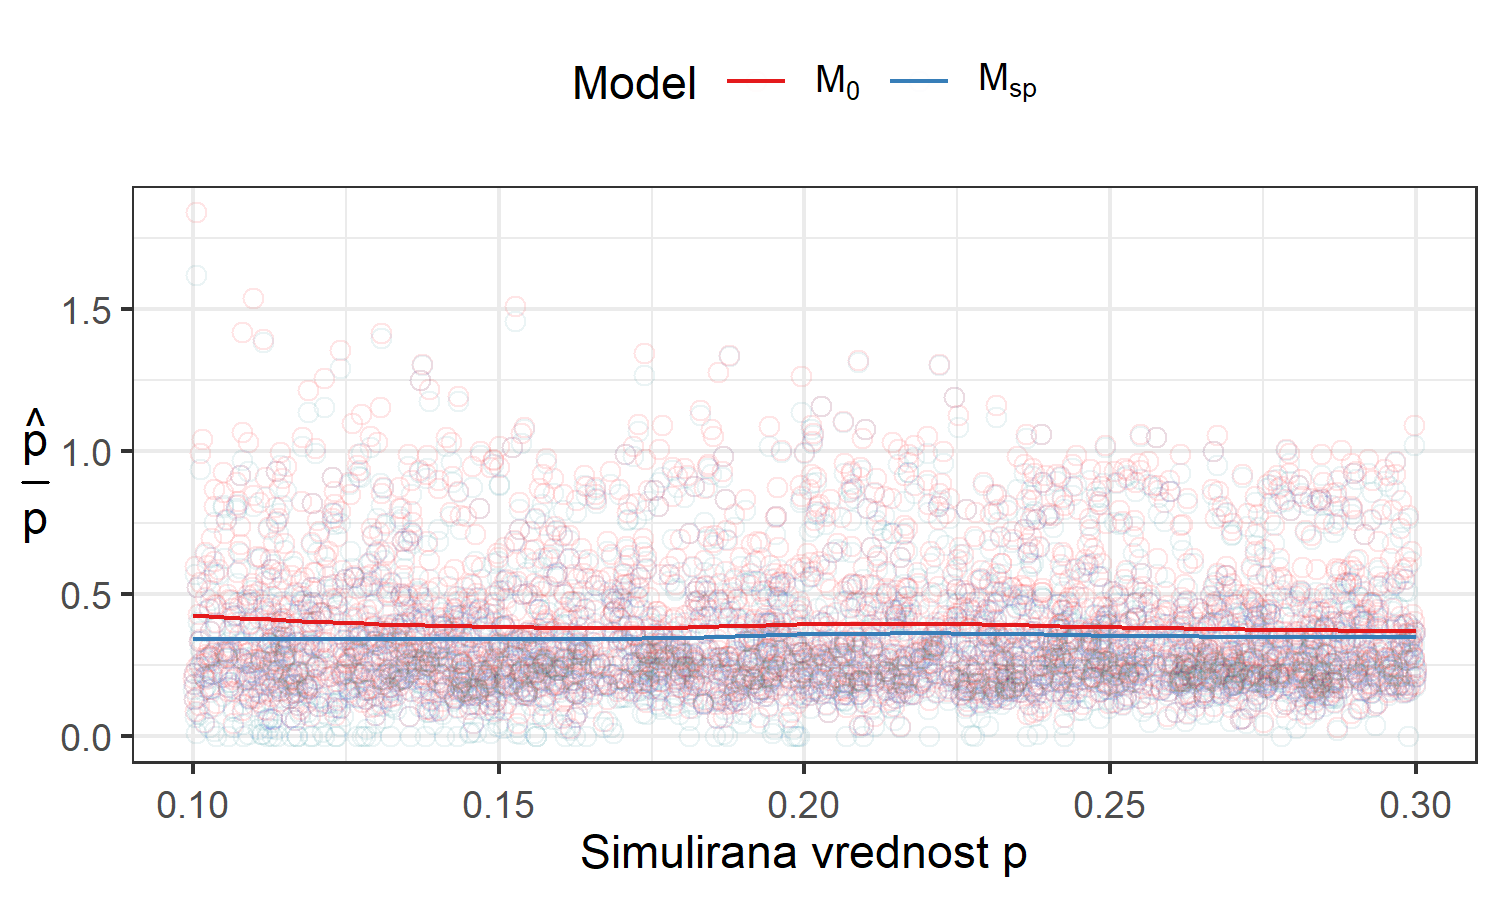
\includegraphics[width=1\linewidth]{C:/Users/romunov/Documents/workspace/doktorat/analiza/figures/N-0a_pristranskost_1_in_sp_ocene_ulovljivosti.png}
  \label{sli:sub3.2}
\end{subfigure}

\caption[Primerjava ocenjene ulovljivosti s simulirano]{Primerjava ocenjene ulovljivosti s simulirano. Povprečna ocena ulovljivosti ($p$) za Hugginsova modela $M_0$ in $M_{sp}$. Na osi $x$ so prikazane simulirane vrednosti $p$, na osi $y$ pa razmerje med ocenjeno in simulirano vrednostjo verjetnosti ulovljivosti. Izračun individualne spremenljivke s pomočjo empirične (zgoraj) in normalne funkcije (spodaj). Ne kaže, da izbira funkcije za izračun individualne spremenljivke bistveno vpliva na oceno parametra $p$.

\medskip

Figure \ref{sli:slika3}: Comparing estimated probability of capture against simulated. Average capture probability estimate from Huggins models $M_0$ and $M_{sp}$. Axis $x$ shows simulated $p$ and $y$ shows ratio between estimated ($\hat{p}$) and simulated value. Upper and lower figures show results where individual covariate has been calculated using empirical and two-dimensional normal functions, respectively. Type of function used does not appear to directly influence the result in a meaningful way.
}
\label{sli:slika3}
\end{figure}

\subsubsection[\bfseries Primerjava verjetnosti ulovljivosti glede na število simuliranih osebkov]{Primerjava verjetnosti ulovljivosti glede na število simuliranih osebkov}
Ocena verjetnosti ulovljivosti ($p$) glede na število simuliranih osebkov kaže podobno sliko (slika \ref{sli:slika4}). V povprečju model, kjer smo uporabili za izračun še individualno spremenljivko ($M_{sp}$), bolj podcenjuje ulovljivost kot model brez nje ($M_0$). Ta razlika je relativno majhna.

Opazili smo tudi trend, da je razkorak med modeloma večji za simulacije z manj osebki za manjše simulirane ulovljivosti. Z večanjem simuliranega parametra p se razlika zmanjšuje tudi za primere z najmanjšim številom simuliranih osebkov. Razlike med simulacijami, kjer smo individualno spremenljivko izračunali s pomočjo empirične ali normalne porazdelitve, so relativno majhne.

\begin{figure}[H]
\centering
\begin{subfigure}[b]{1\textwidth}
  \centering
  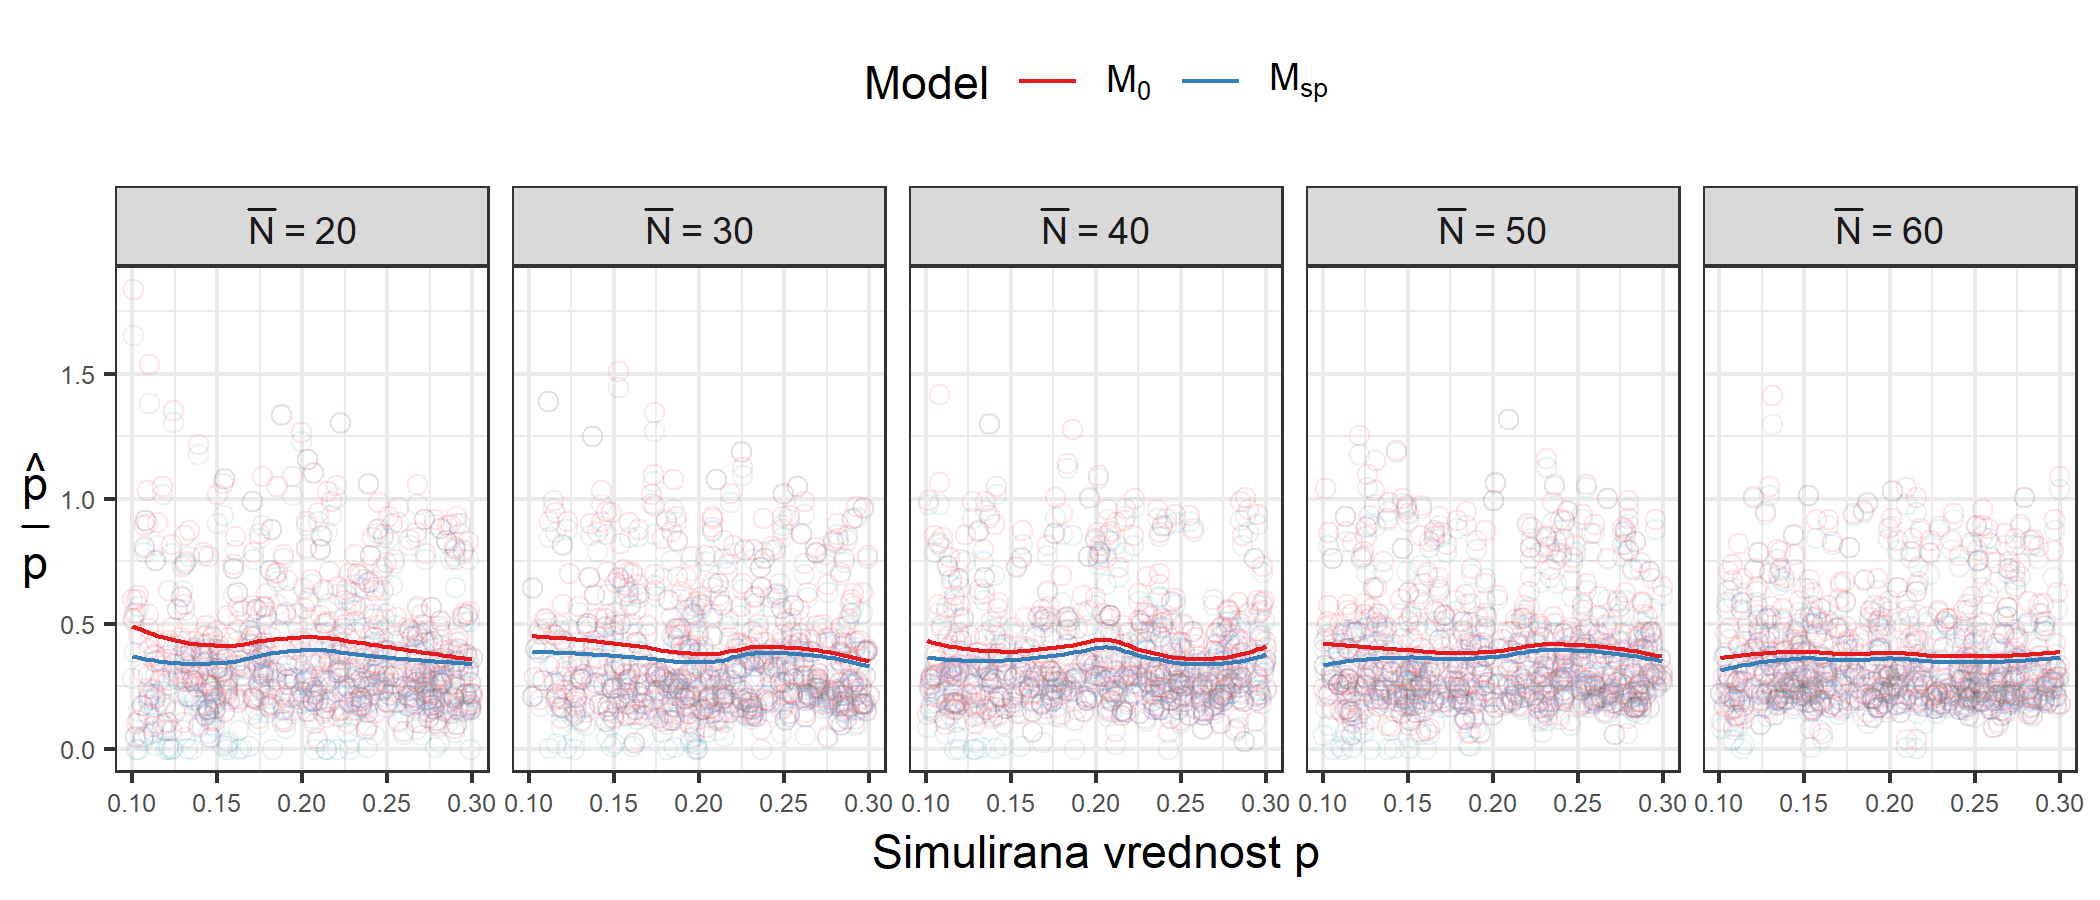
\includegraphics[width=1\linewidth]{C:/Users/romunov/Documents/workspace/doktorat/analiza/figures/E-0b_pristranskost_p1_in_psp_glede_na_st_walkerjev.png}

  \label{sli:sub4.1}
\end{subfigure}

\begin{subfigure}[b]{1\textwidth}
  \centering
  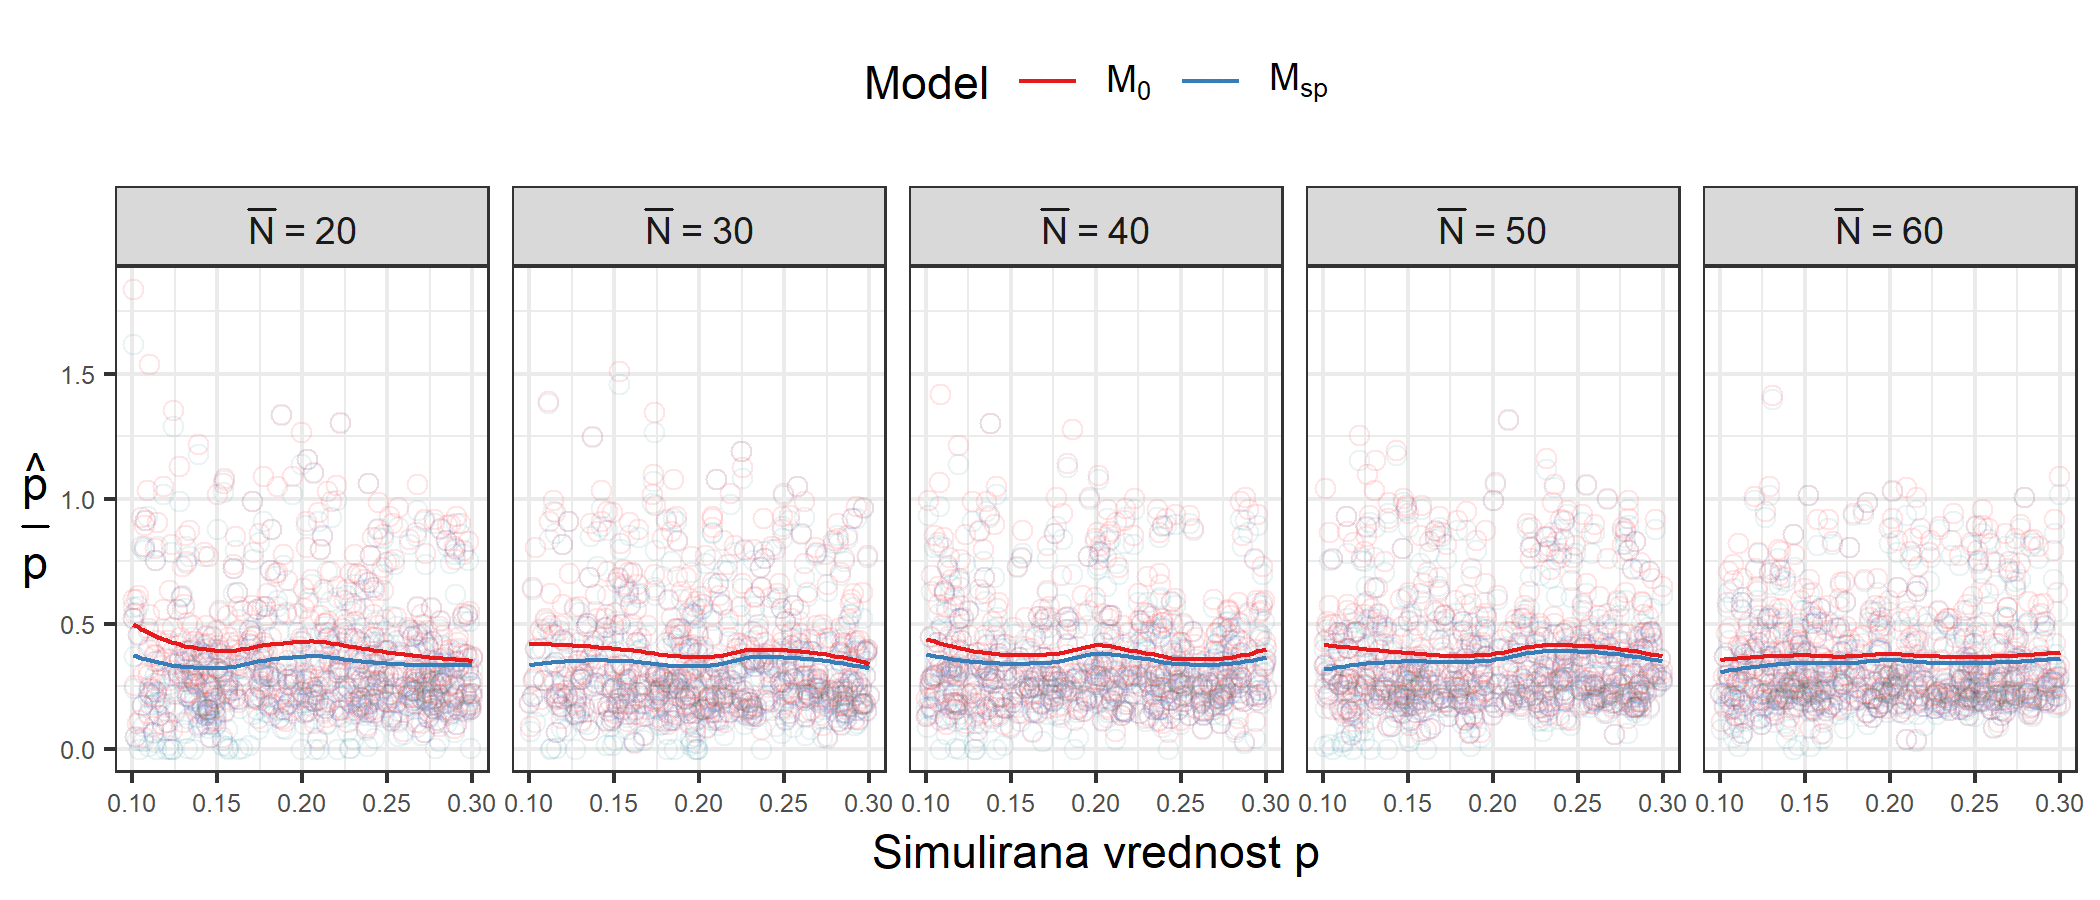
\includegraphics[width=1\linewidth]{C:/Users/romunov/Documents/workspace/doktorat/analiza/figures/N-0b_pristranskost_p1_in_psp_glede_na_st_walkerjev.png}
  \label{sli:sub4.2}
\end{subfigure}

\caption[Primerjava ocenjene ulovljivosti s simulirano glede na število simuliranih osebkov]{Primerjava ocenjene ulovljivosti s simulirano glede na število simuliranih osebkov. Točke prikazujejo razmerje med oceno ulovljivosti ($\hat{p}$) in simulirano vrednostjo glede na povprečno število generiranih osebkov znotraj območja vzorčenja. Na $x$ osi so prikazane simulirane vrednosti ulovljivosti, na $y$ osi pa razmerje med ocenjeno in simulirano vrednostjo. Okenca prikazujejo podatke glede na povprečno število simuliranih osebkov znotraj območja vzorčenja. Zgornja slika prikazuje podatke, kjer smo individualno spremenljivko ocenili s pomočjo empirične porazdelitve, spodnja pa podatke za simulacije, kjer smo individualno spremenljivko izračunali s pomočjo normalne porazdelitve.

\medskip

Figure \ref{sli:slika4}: Comparing estimate probability of capture to simulated by number of simulated individuals. Figure shows ratio between estimated ($\hat{p}$) and simulated ($p$) probability of capture on the $y$ axis given the simulated values on $x$ axis. Number of individuals generated within the sampling polygon per simulation is divided by facets. Upper and lower figures represent results where individual covariate has been calculated using empirical and two-dimensional normal distribution, respectively.}
\label{sli:slika4}
\end{figure}

\subsubsection[\bfseries Primerjava ulovljivosti glede na razmerje velikosti domačega okoliša in območja vzorčenja]{Primerjava ulovljivosti glede na razmerje velikosti domačega okoliša in območja vzorčenja}
S slike \ref{sli:slika5} je razvidno, da je vpliv zelo velik. Ko je razmerje velikosti domačega okoliša in velikosti območja vzorčenja majhno (majhen domač okoliš v primerjavi z območjem vzorčenja), je ocena parametra relativno zanesljiva. Z večanjem razmerja med domačim okolišem in območjem vzorčenja pa se zanesljivost ocene poslabšuje in se celo spusti pod globalno povprečje.

Sodeč po rezultatih s slike \ref{sli:slika5}, ne moremo sklepati, da ima število generiranih osebkov v povezavi z razmerjem velikosti domačega okoliša in območja vzorčenja bistven vpliv na oceno ulovljivosti, oziroma je vpliv neznaten. Razlike med simulacijami, kjer smo spreminjali funkcijo za izračun individualne spremenljivke, so majhne oz. jih v praktičnem smislu ni.

\begin{figure}[H]
\centering
\begin{subfigure}[b]{1\textwidth}
  \centering
  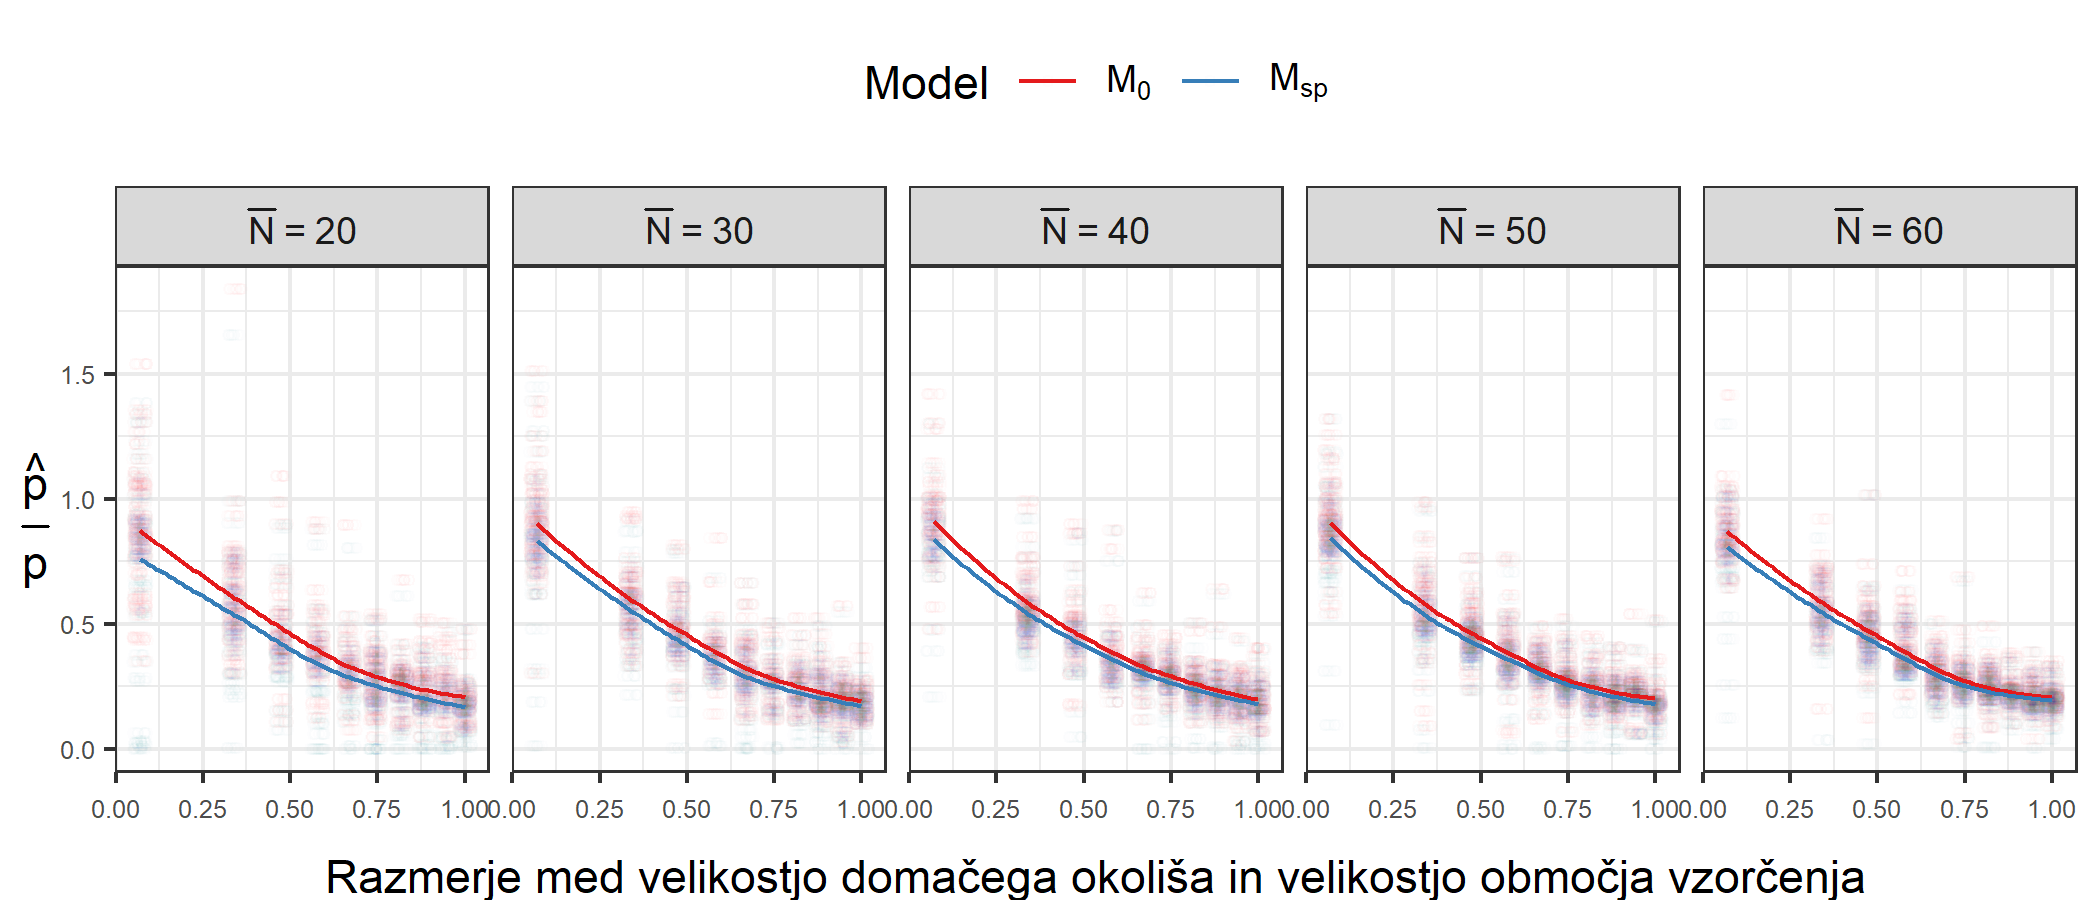
\includegraphics[width=1\linewidth]{C:/Users/romunov/Documents/workspace/doktorat/analiza/figures/E-0f_pristranskost_p_glede_na_sap_hr_ratio_po_st_gen_walkerjev_brez_popravka.png}

  \label{sli:sub5.1}
\end{subfigure}

\begin{subfigure}[b]{1\textwidth}
  \centering
  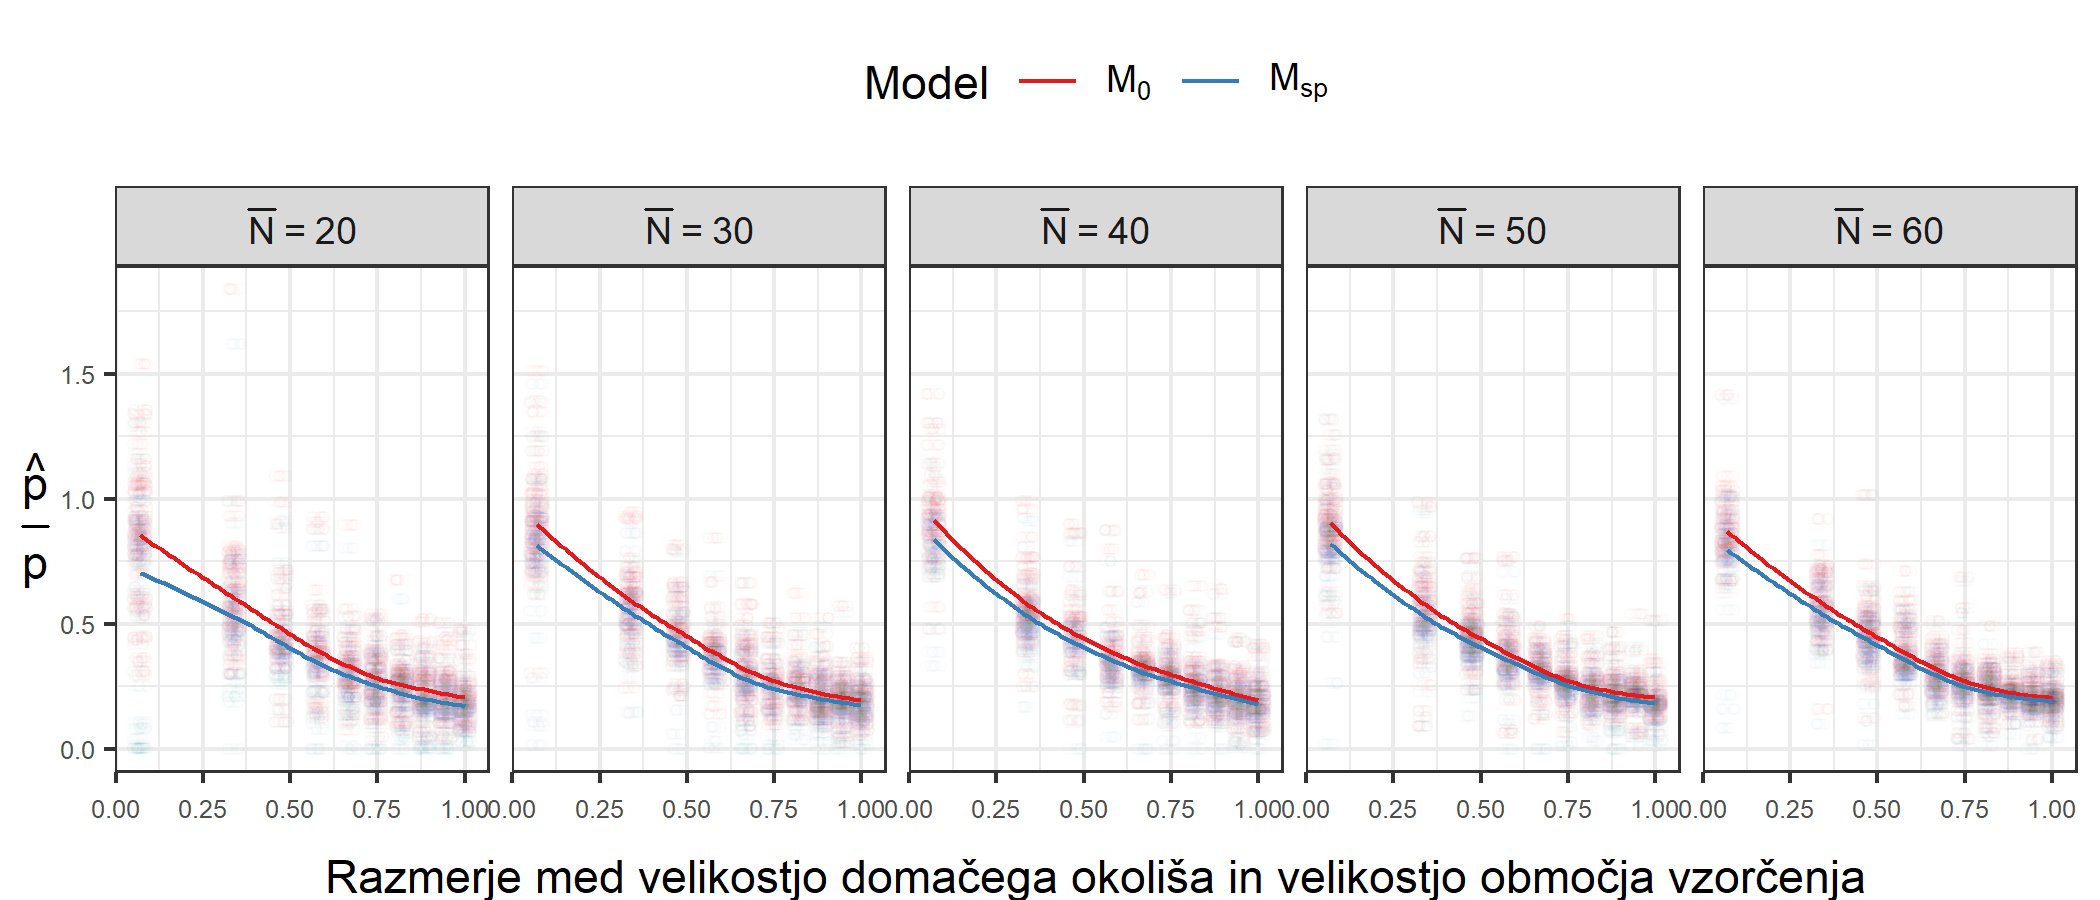
\includegraphics[width=1\linewidth]{C:/Users/romunov/Documents/workspace/doktorat/analiza/figures/N-0f_pristranskost_p_glede_na_sap_hr_ratio_po_st_gen_walkerjev_brez_popravka.png}
  \label{sli:sub5.2}
\end{subfigure}

\caption[Vpliv razmerja med ocenjeno in pravo ulovljivostjo v povezavi z razmerjem velikosti domačega okoliša in vzorčenega območja]{Vpliv razmerja med ocenjeno in pravo ulovljivostjo v povezavi z razmerjem velikosti domačega okoliša in vzorčenega območja. Zgornja slika prikazuje rezultate simulacij, kjer smo individualno spremenljivko izračunali s pomočjo empirične porazdelitve, spodnja pa za izračune s pomočjo normalne porazdelitve. Okenca predstavljajo povprečno število osebkov, ki smo jih generirali znotraj območja vzorčenja.

\medskip

Figure \ref{sli:slika5}: Influence of ratio between estimated and simulated probability of capture by ratio of home range size and sampling polygon size. Influence of ratio between home range size and sampling polygon size (on $x$) on estimate of probability of capture depicted as ratio between estimated and simulated probabilities of capture ($y$ axis). Facets depict simulations based on number of simulated individuals within the sampling polygon. Upper and lower images represent simulations where individual covariate was calculated using empirical and two-dimensional normal distribution, respectively.
}
\label{sli:slika5}
\end{figure}

Razmerje med površinama domačega okoliša in območja vzorčenja ima na pristranskost ocene parametra $p$ velik vpliv. Na sliki \ref{sli:slika6} je prikazano, kako se pristranskost ocene parametra $p$ spreminja z razmerjem površin domačega okoliša in vzorčenega območja glede na število generiranih osebkov in število odlovnih intervalov. Povprečji ocen obeh Hugginsovih modelov konvergirata z večanjem razmerja, kjer več simuliranih osebkov pomeni bolj podobno (in pristransko) oceno med modeloma. Podoben vpliv ima tudi število odlovnih intervalov, ki poleg tega vpliva tudi na variabilnost ocen. Več kot je odlovnih intervalov, manjša je variabilnost v oceni. S slike \ref{sli:slika6} ne moremo trditi, da smo zaznali bistvene razlike med simulacijami, kjer smo uporabili za izračun normalno ali empirično funkcijo.

\begin{figure}[H]
\centering
\begin{subfigure}[b]{0.8\textwidth}
  \centering
  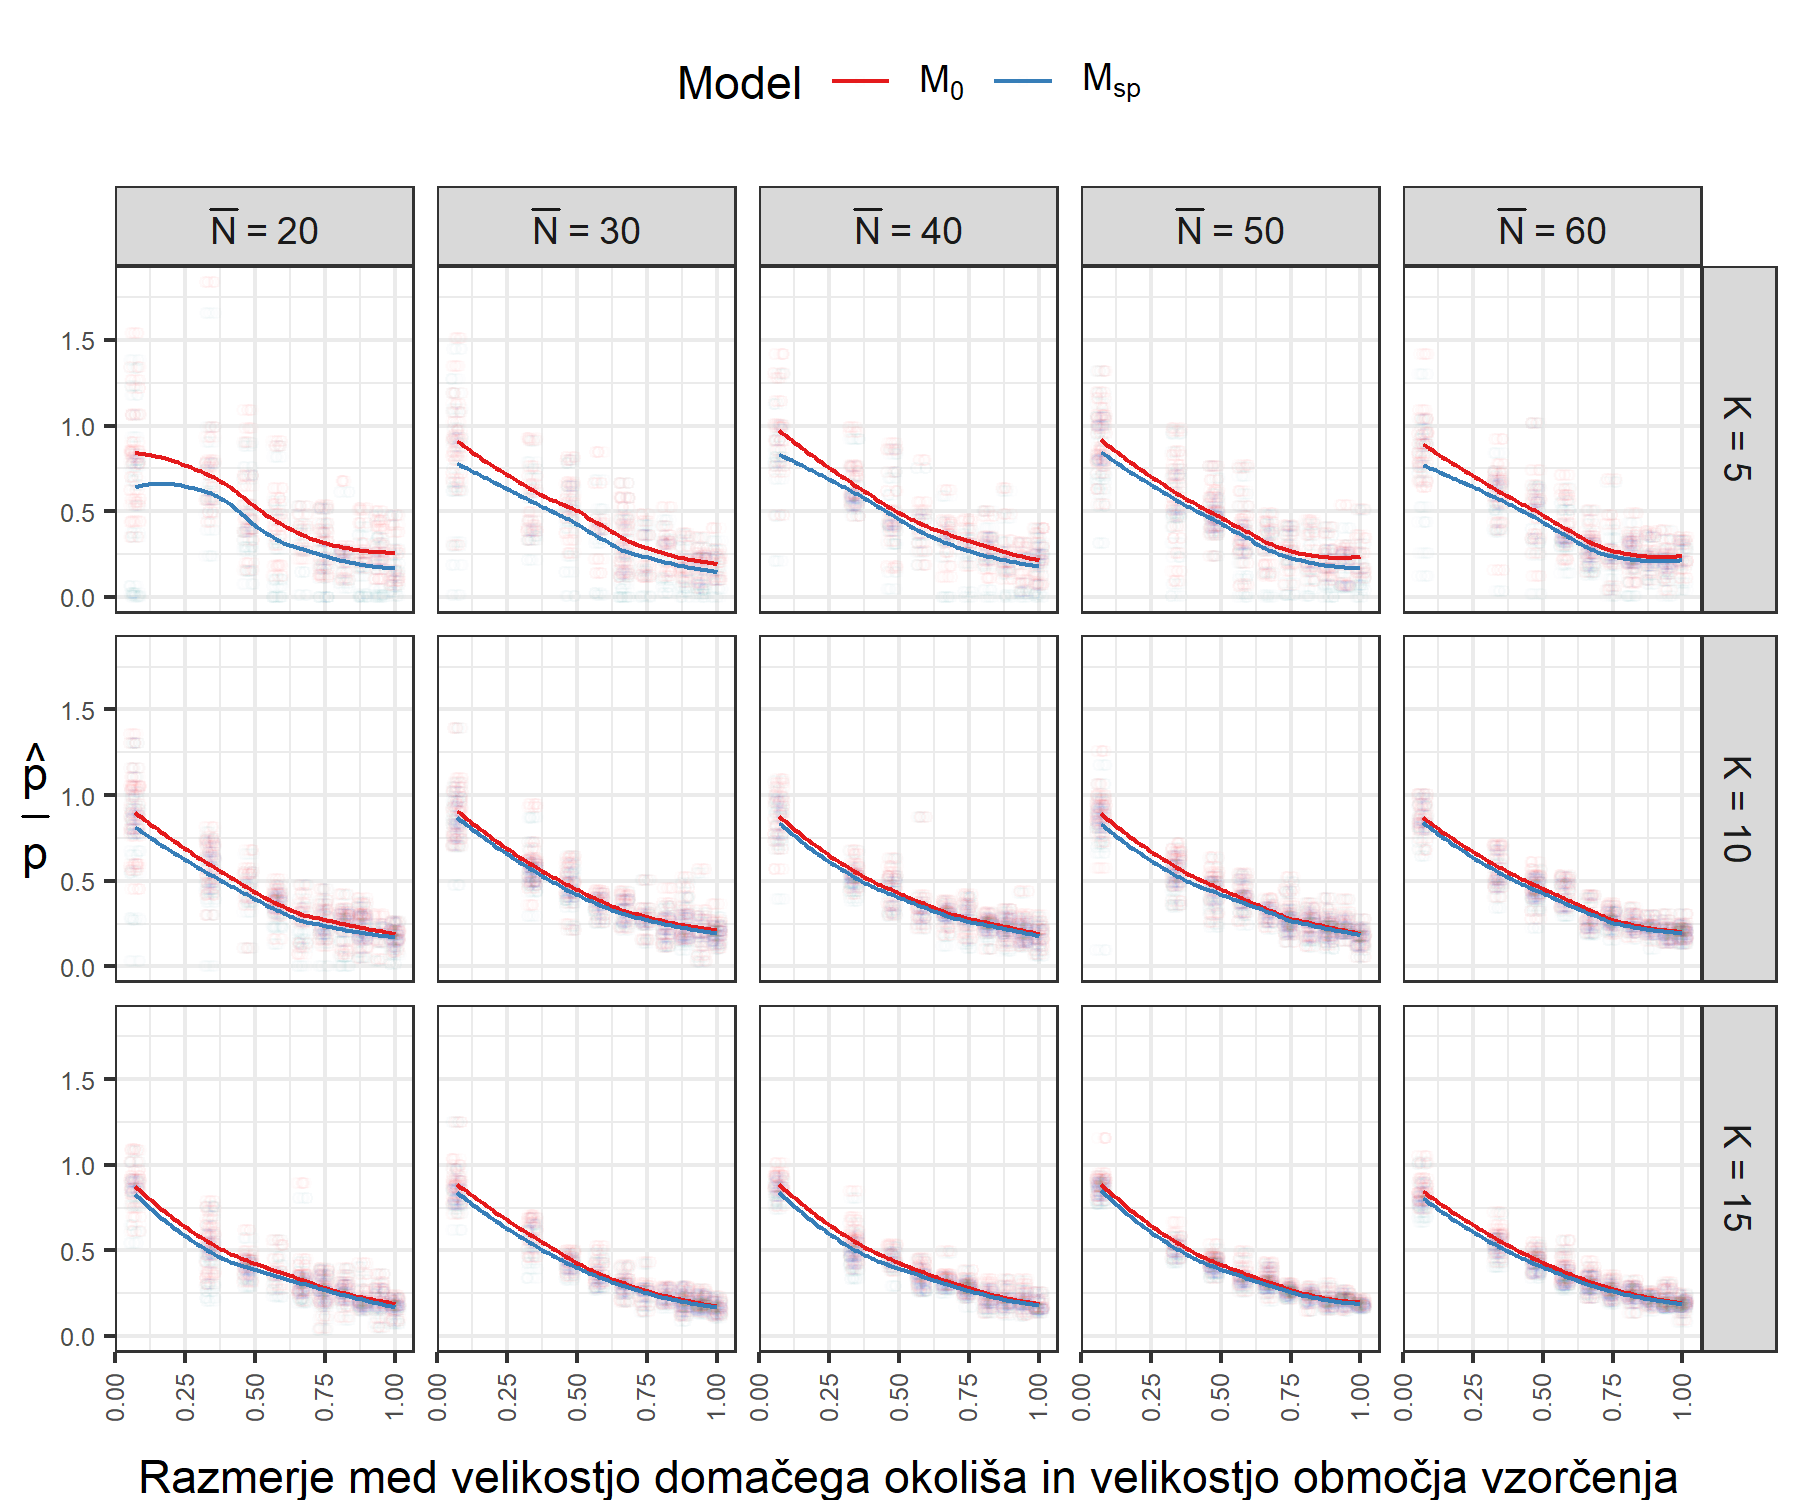
\includegraphics[width=1\linewidth]{C:/Users/romunov/Documents/workspace/doktorat/analiza/figures/E-0h_pristranskost_p_glede_sap_hr_razmerje_glede_na_st_walkerjev_in_st_sessionov.png}
  \label{sli:sub6.1}
\end{subfigure}

\begin{subfigure}[b]{0.8\textwidth}
  \centering
  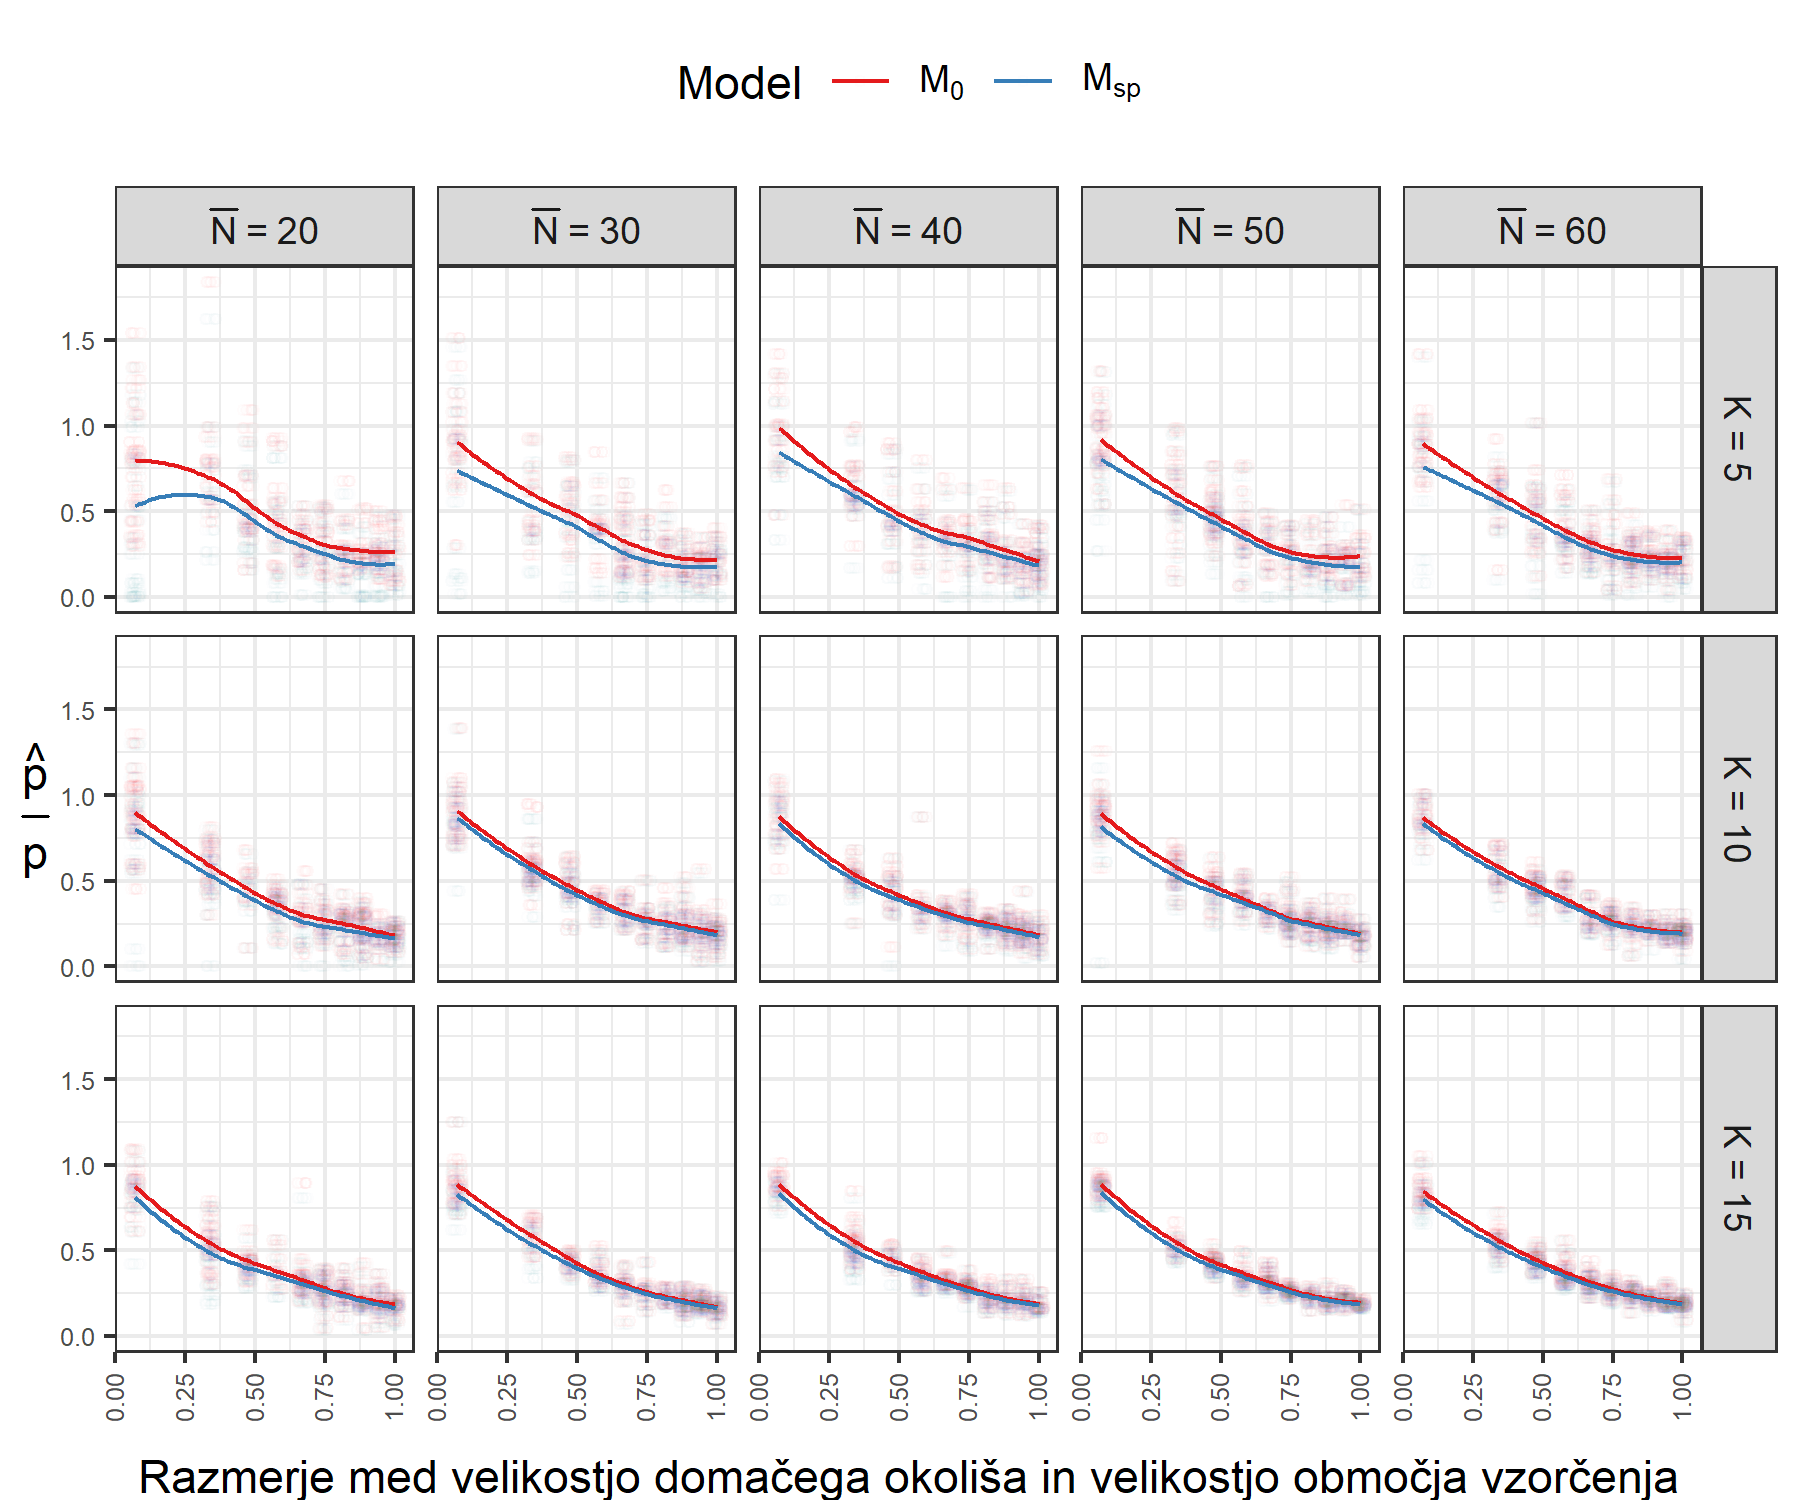
\includegraphics[width=1\linewidth]{C:/Users/romunov/Documents/workspace/doktorat/analiza/figures/N-0h_pristranskost_p_glede_sap_hr_razmerje_glede_na_st_walkerjev_in_st_sessionov.png}
  \label{sli:sub6.2}
\end{subfigure}
\caption[Prikaz pristranskosti ocene ulovljivosti glede na razmerje površin domačega okoliša in območja vzorčenja v povezavi s številom simuliranih osebkov in odlovnih intervalov]{Prikaz pristranskosti ocene ulovljivosti ($\hat{p}$) glede na razmerje površin domačega okoliša in območja vzorčenja v povezavi s številom simuliranih osebkov (stolpci) in odlovnih intervalov (vrstice). Na zgornji sliki so prikazani rezultati simulacij, kjer smo za izračun individualne spremenljivke uporabili empirično, na spodnji pa normalno funkcijo. Z večanjem števila simuliranih osebkov se veča pristranskost in manjša razlika v oceni parametra. Podobno sliko vidimo z večanjem števila odlovnih intervalov (vrstice), kjer poleg višanja pristranskosti in konvergence povprečij modelov opazimo tudi zmanjševanje variance ocene.\\
Se nadaljuje
}
\label{sli:slika6}
\end{figure}

\begin{figure}\ContinuedFloat
\caption*{nadaljevanje Figure \ref{sli:slika6}: Depiction of bias as ratio of estimated probability of capture and simulated value against ratio of home range area and sampling polygon area by number of simulated individuals and sampling sessions. Data has been additionally sliced according to number of sampling occasions ($K$, facets in rows) and number of simulated individuals within sampling polygon ($\bar{N}$, facets in columns). Bias increases with increased ratio between home range size and sampling polygon size. On average, means of models converge and are highly biased for large ratios of home range size and sampling polygon size. By increasing number of sampling sessions, decrease in variance of estimates is apparent.}
\end{figure}

\subsection{GOSTOTA}
Simulirano gostoto smo izračunali kot število centroidov (osebkov) znotraj površine, kjer smo jih simulirali. S pomočjo modelov Huggins in TIRM smo dobili oceno številčnosti znotraj območja vzorčenja. Ker osebki niso bili omejeni na območje vzorčenja in so prehajali njegove meje, smo dejansko ocenili velikost superpopulacije, katere prostorska omejenost ni nedvoumno določena. Na podlagi ocenjenega števila osebkov in velikosti vzorčenega območja smo izračunali gostoto te superpopulacije.

Za izračun gostote smo uporabili tudi razširjeno območje vzorčenja. Območje smo razširili tako, da smo polmer povečali za določeno razdaljo. Razdaljo smo izbrali kot percentil parne razdalje iz funkcije, ki smo jo ali prilegli podatkom (empirična funkcija) ali pa izračunali na podlagi simuliranih parametrov (dvorazsežna normalna porazdelitev). Gostoto smo izračunali glede na območje, povečano za standardni odklon polmera simuliranega območja gibanja osebka (hr), za percentil porazdelitve (50-99) oz. za najdaljšo prehojeno razdaljo (effect) v posamezni simulaciji. Spodnji rezultati so podani kot razmerje med ocenjeno in pravo gostoto. Ker gre za razmerje, kjer je prava gostota v imenovalcu, se bodo v primeru nepristransko ocenjene gostote vrednosti nahajale blizu 1.


\subsubsection[\bfseries Razlike v gostoti glede na število simuliranih osebkov in funkcij za izračun individualne spremenljivke]{Razlike v gostoti glede na število simuliranih osebkov in funkcij za izračun individualne spremenljivke}
Na sliki \ref{sli:slika6} so prikazani rezultati izračuna gostot. Na sliki uporabimo kazalnik, ki je z gostoto povezan kot razmerje med gostoto, izračunano iz ocenjene velikosti populacije, in gostoto, izračunano iz simulirane velikosti populacije ($\hat{D}/D$).

Opazimo razlike med simulacijami, kjer smo uporabili empirično in normalno porazdelitev za izračun individualne spremenljivke. Razlike so predvsem v primerih, kjer smo območje vzorčenja povečali za razdaljo od 50. do 99. percentila. Pristranskost kazalnika se v odvisnosti od razmerja domačega okoliša in vzorčenega območja povečuje hitreje za primere, ko smo za izračun individualne spremenljivke uporabili empirično porazdelitev.

Pristranskost kazalnika v primeru nepovečanega območja hitro narašča z večanjem razmerja med velikostjo domačega okoliša in velikostjo območja vzorčenja podobno za oba načina izračuna individualne spremenljivke.

Z manjšanjem razmerja med površino domačega okoliša in območja vzorčenja se pristranskost v povprečju zmanjšuje. Za primere, kjer smo za izračun individualne spremenljivke uporabili empirično funkcijo, je gladilka za večja povečanja razmerja bolj konkavne oblike, s povečevanjem površine vzorčenega območja za izračun gostote pa se pristranskost v splošnem zmanjšuje.
Pri simulacijah, kjer smo za izračun individualne spremenljivke uporabili normalno porazdelitev, je konkavnost gladilke možno opaziti le za primere, kjer smo območje vzorčenja povečali za najdaljšo prehojeno razdaljo (zadnji stolpec).
Za oba načina izračuna individualnih spremenljivk pa velja, da se povečanje površine vzorčenega območja pozna najmanj za tiste simulacije, kjer je bilo razmerje med velikostjo domačega okoliša in velikostjo vzorčenega območja najmanjše.

Povečevanje števila simuliranih osebkov prispeva predvsem k zmanjšanju variabilnosti ocen velikosti populacij in posledično k manjši variabilnosti gostot. Variabilnost je za veliko večino primerov najmanjša za simulacije, kjer je razmerje med velikostjo domačega okoliša in velikostjo vzorčenega območja najmanjša.

Razlike med modeli so med scenariji primerljive. Najbolj precenjene rezultate da model TIRM, manj $M_{sp}$ in najmanj $M_0$. Razlike med modeli izginejo predvsem na račun povečanja razmerja med površinama domačega okoliša in območja vzorčenja.

\begin{figure}[H]
  \centering
  \begin{subfigure}[b]{1\textwidth}
    \centering
    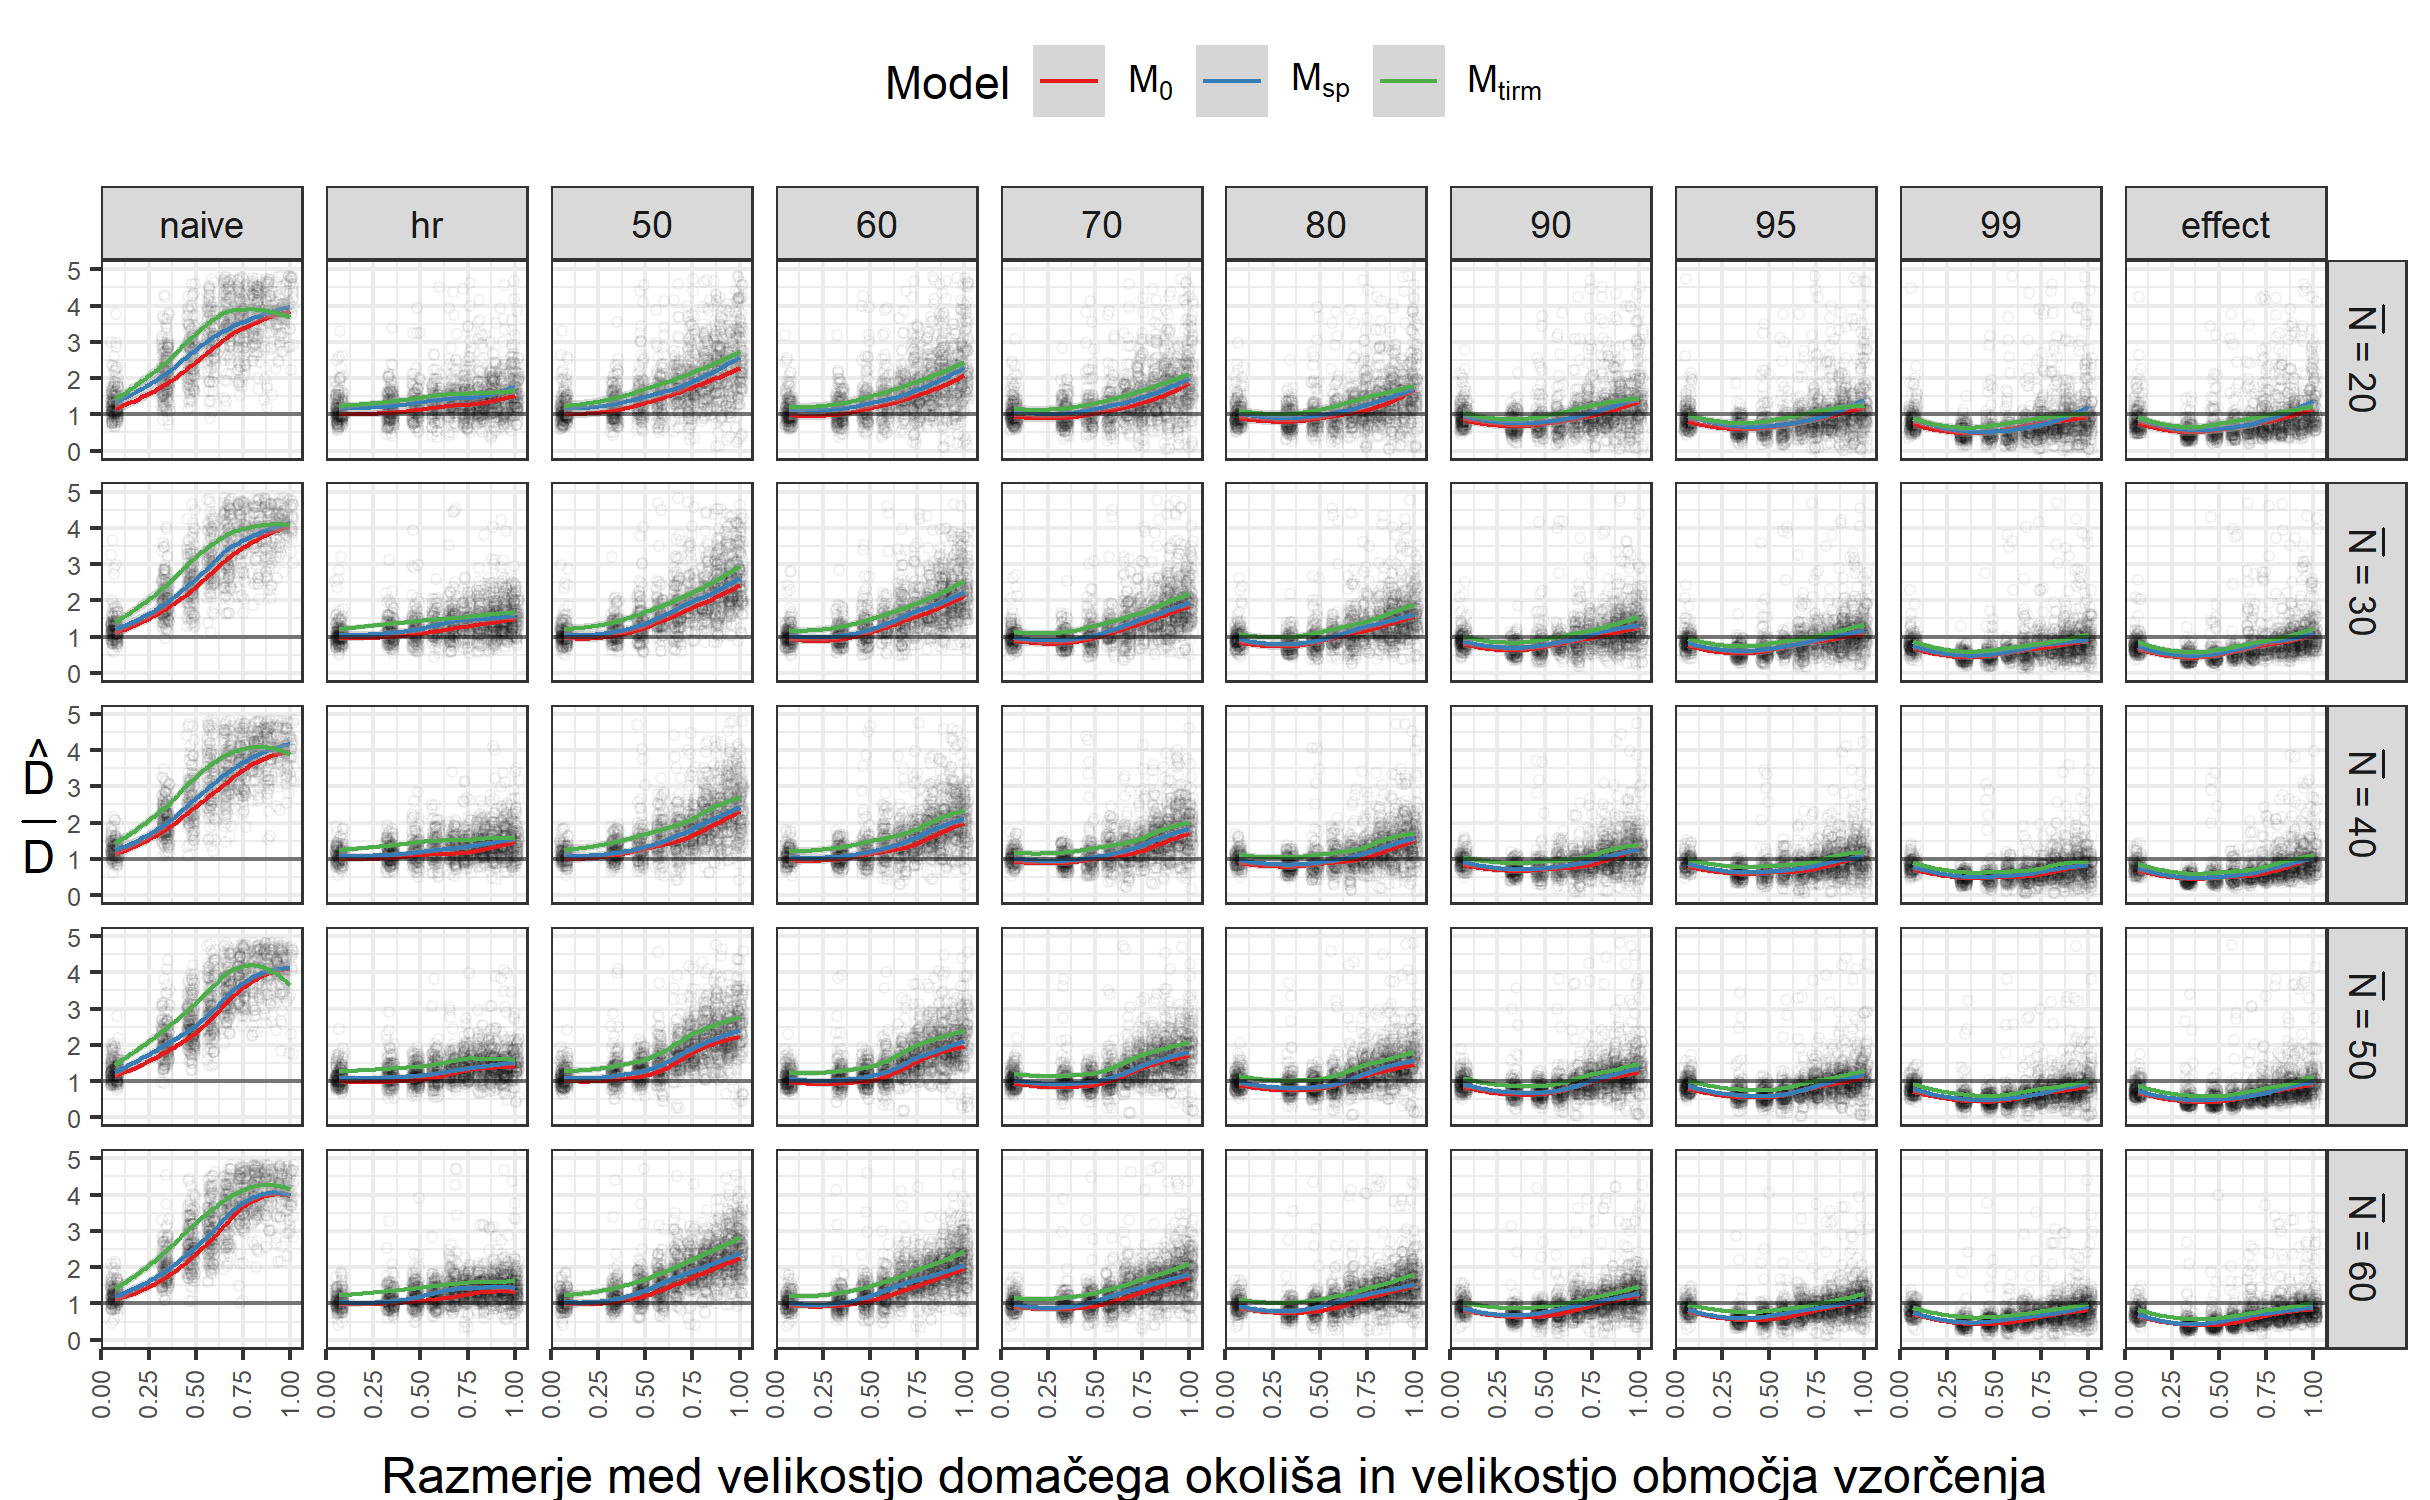
\includegraphics[width=1\linewidth]{C:/Users/romunov/Documents/workspace/doktorat/analiza/figures/E-1a_gostota_gled_na_razmerje_hr_sap_po_correction_type_in_st_gen_walk.png}
    \label{sli:sub7.1}
  \end{subfigure}

  \begin{subfigure}[b]{1\textwidth}
    \centering
    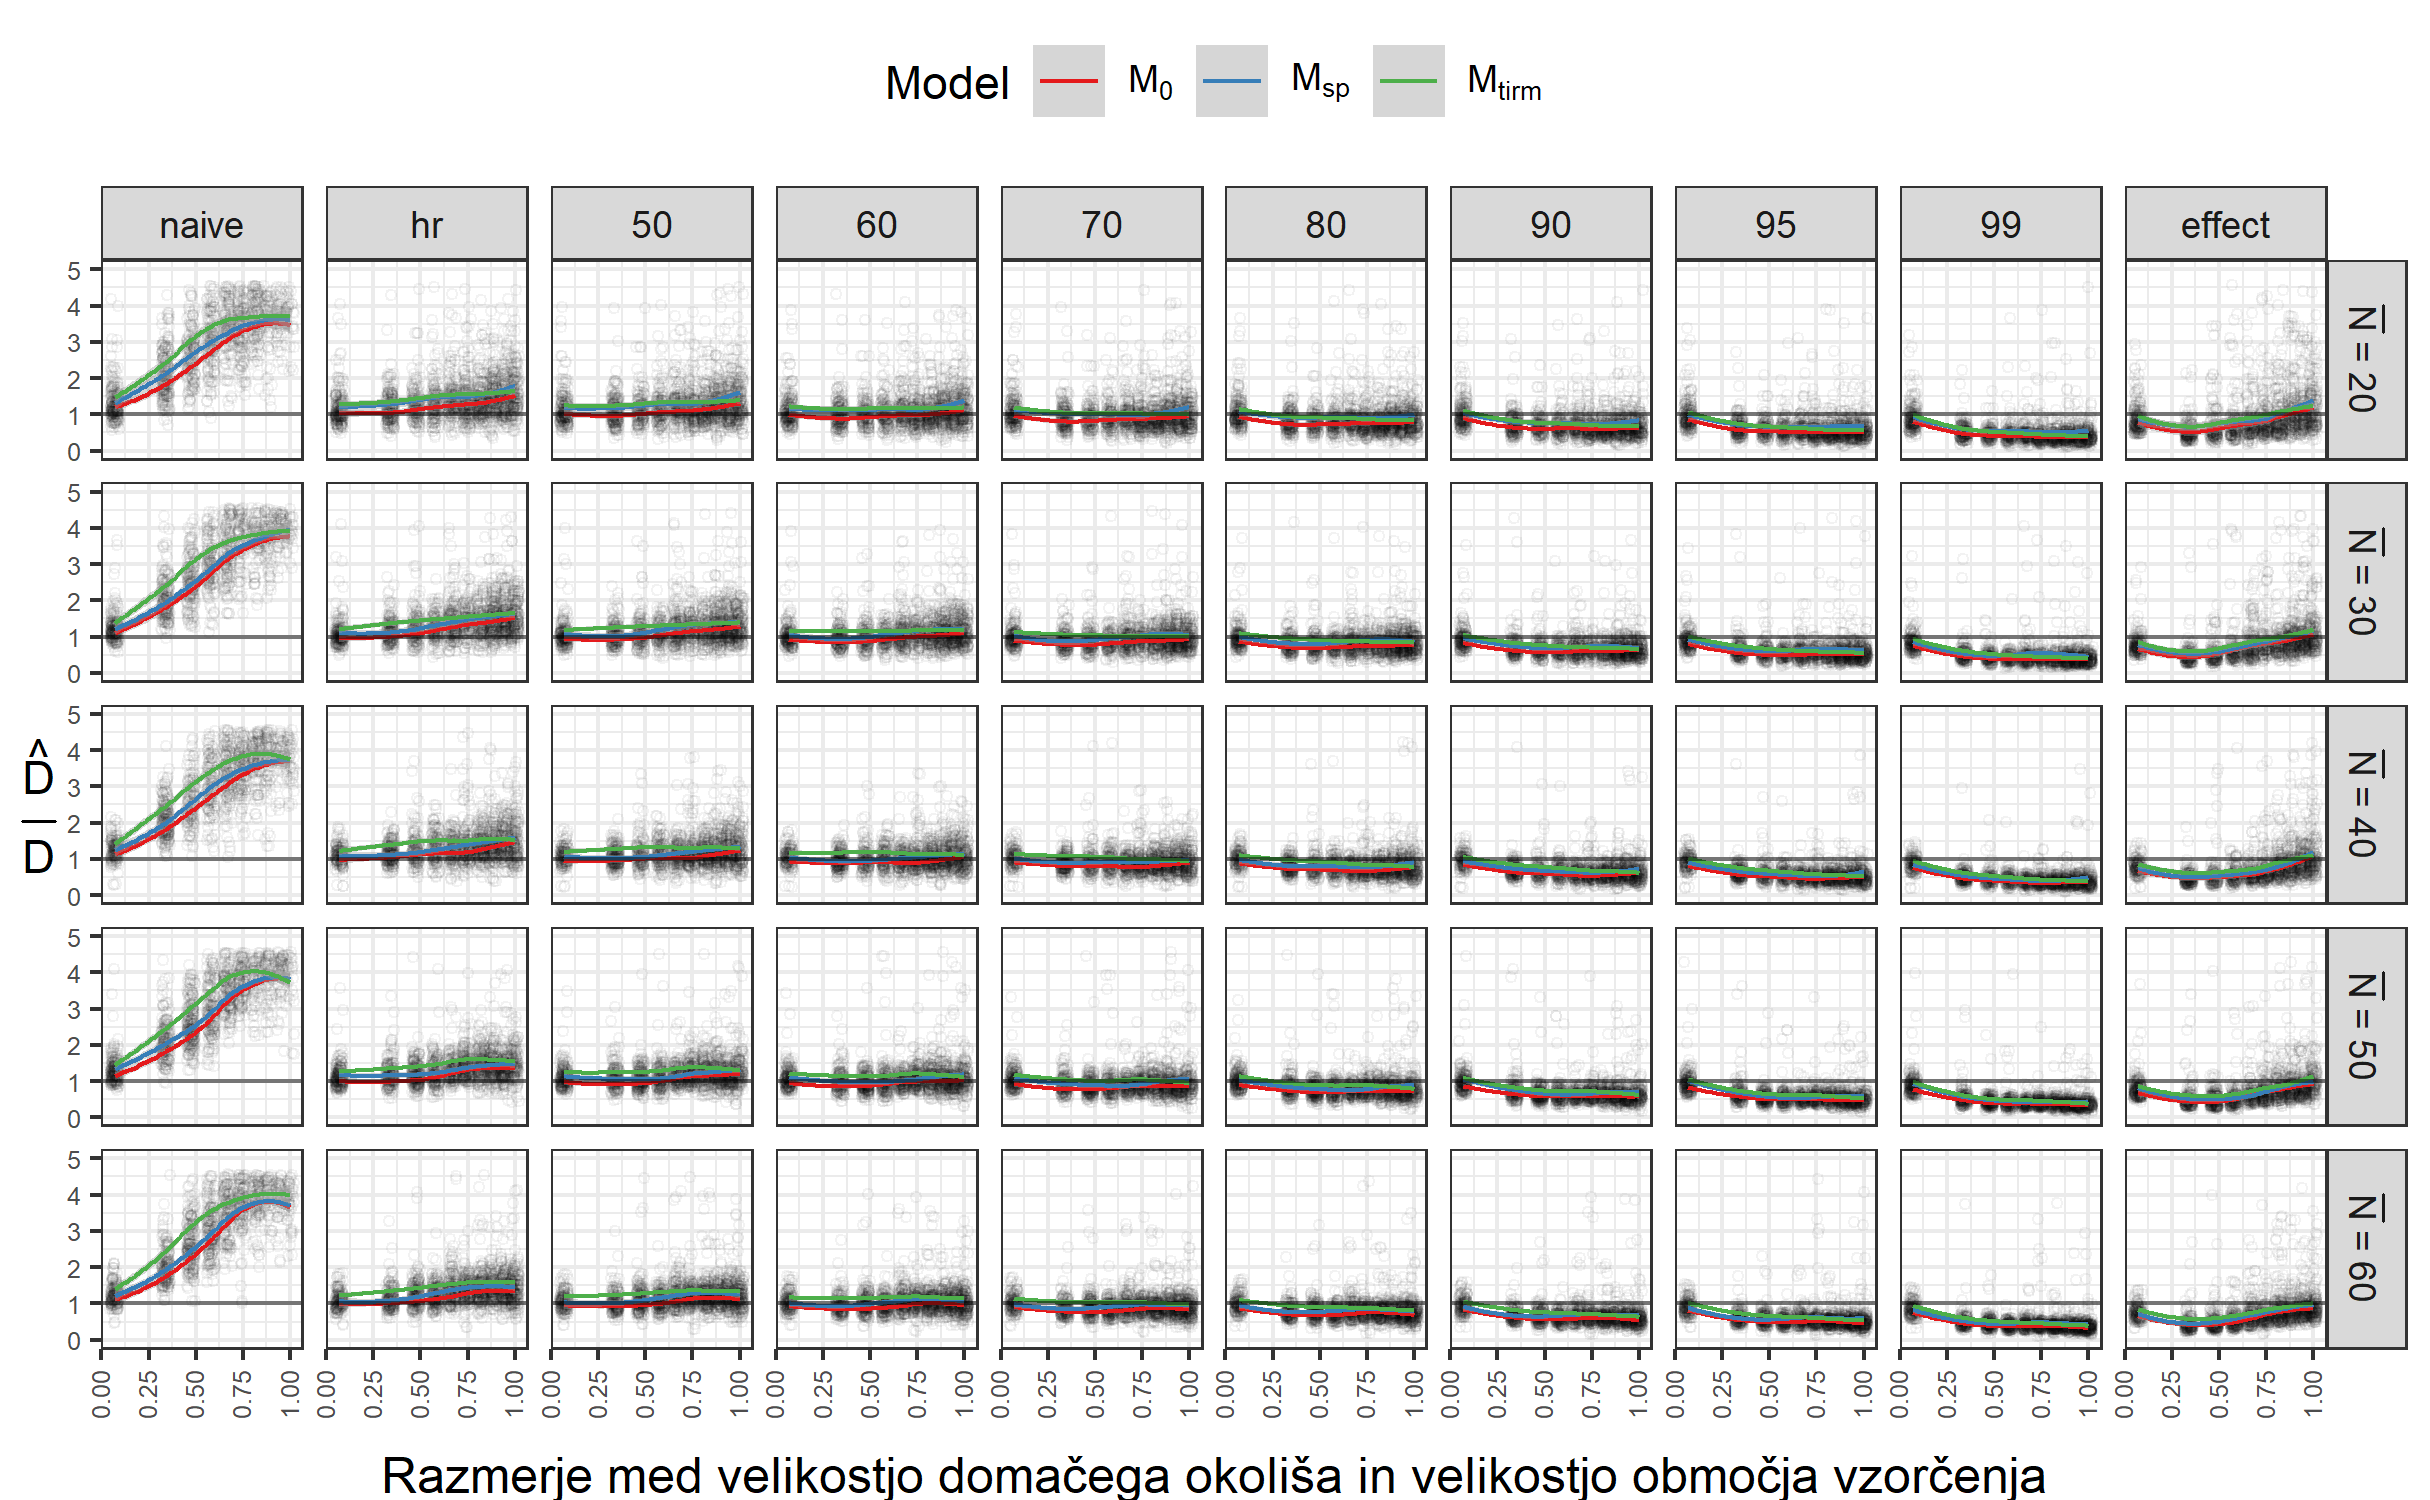
\includegraphics[width=1\linewidth]{C:/Users/romunov/Documents/workspace/doktorat/analiza/figures/N-1a_gostota_gled_na_razmerje_hr_sap_po_correction_type_in_st_gen_walk.png}
    \label{sli:sub7.2}
  \end{subfigure}
  \caption[Prikaz kazalnika gostot]{Prikaz kazalnika gostot ($\hat{D}/D$) glede na razmerje velikosti domačega okoliša in velikosti območja vzorčenja. Na zgornji sliki so prikazani rezultati za simulacije, kjer smo za izračun individualne spremenljivke uporabili empirično porazdelitev, na spodnji pa za simulacije, kjer smo uporabili dvorazsežno normalno porazdelitev. Stolpci oken ponazarjajo razširitev vzorčenega območja, vrstice pa povprečno število simuliranih osebkov znotraj območja vzorčenja, na katerih smo izvedli vzorčenje ter posledično izračun velikosti populacije in gostote. Pri izračunu smo uporabili tri modele, dve različici Hugginsovega modela ($H_0$, $H_{sp}$), kjer smo ulovljivost modelirali glede na individualno spremenljivko, in TIRM, ki predpostavlja dve skupini z različno ulovljivostjo.\\
  Se nadaljuje}
  \label{sli:slika7}
\end{figure}
\begin{figure}\ContinuedFloat
\caption*{nadaljevanje Figure \ref{sli:slika7}: Index of density estimates. Index of density estimates ($\hat{D}/D$) on $y$ axis by ratio of home range size and sampling polygon area ($x$ axis). Upper and lower images represent simulations where individual covariate was calculated using empirical and two-dimensional normal distributions, respectively. Facets in columns represent the sampling polygon expanded by a given measure and rows represent the mean number of simulated individuals within the sampling polygon. Three models are used to calculate population size, two Huggins models $M_0$ and $M_{sp}$ (equal capture probability and probability that depends on individual covariate) and a TIRM model that assumes two groups with each having its own capture probability.}
\end{figure}

\subsubsection[\bfseries Razlike v gostoti glede na funkcijo za izračun individualne spremenljivke, število odlovnih intervalov ter število simuliranih osebkov]{Razlike v gostoti glede na funkcijo za izračun individualne spremenljivke, število odlovnih intervalov ter število simuliranih osebkov}
Na slikah \ref{sli:slika7} in \ref{sli:slika8} smo podatke s slike \ref{sli:slika6} prikazali tako, da so podatki razdeljeni na odlovne intervale ($K = [5, 10, 15]$). Prikaz glede na število odlovnih intervalov nam je dal predvsem vpogled v spremembo variabilnosti. Pri simulacijah z najmanj odlovnimi intervali ($K = 5$) je varianca večja kot pri tistih z več odlovnimi intervali ($K = [10, 15]$). Pri slednjih že opazimo prevladujoč vzorec v povprečju kazalnika za vse modele glede na popravke velikosti območja vzorčenja (stolpci) in povprečno število simuliranih osebkov znotraj območja vzorčenja (vrstice). Vpliv povečanja površine vzorčenega območja se opazi predvsem za simulacije, kjer je razmerje med velikostjo domačega okoliša in velikostjo vzorčenega območja relativno veliko. Na simulacije, kjer je to razmerje relativno majhno, povečanje območja vzorčenja pri pristranskosti ne kaže očitnega učinka.

\begin{figure}[H]
  \centering
  \begin{subfigure}[b]{1\textwidth}
    \centering
    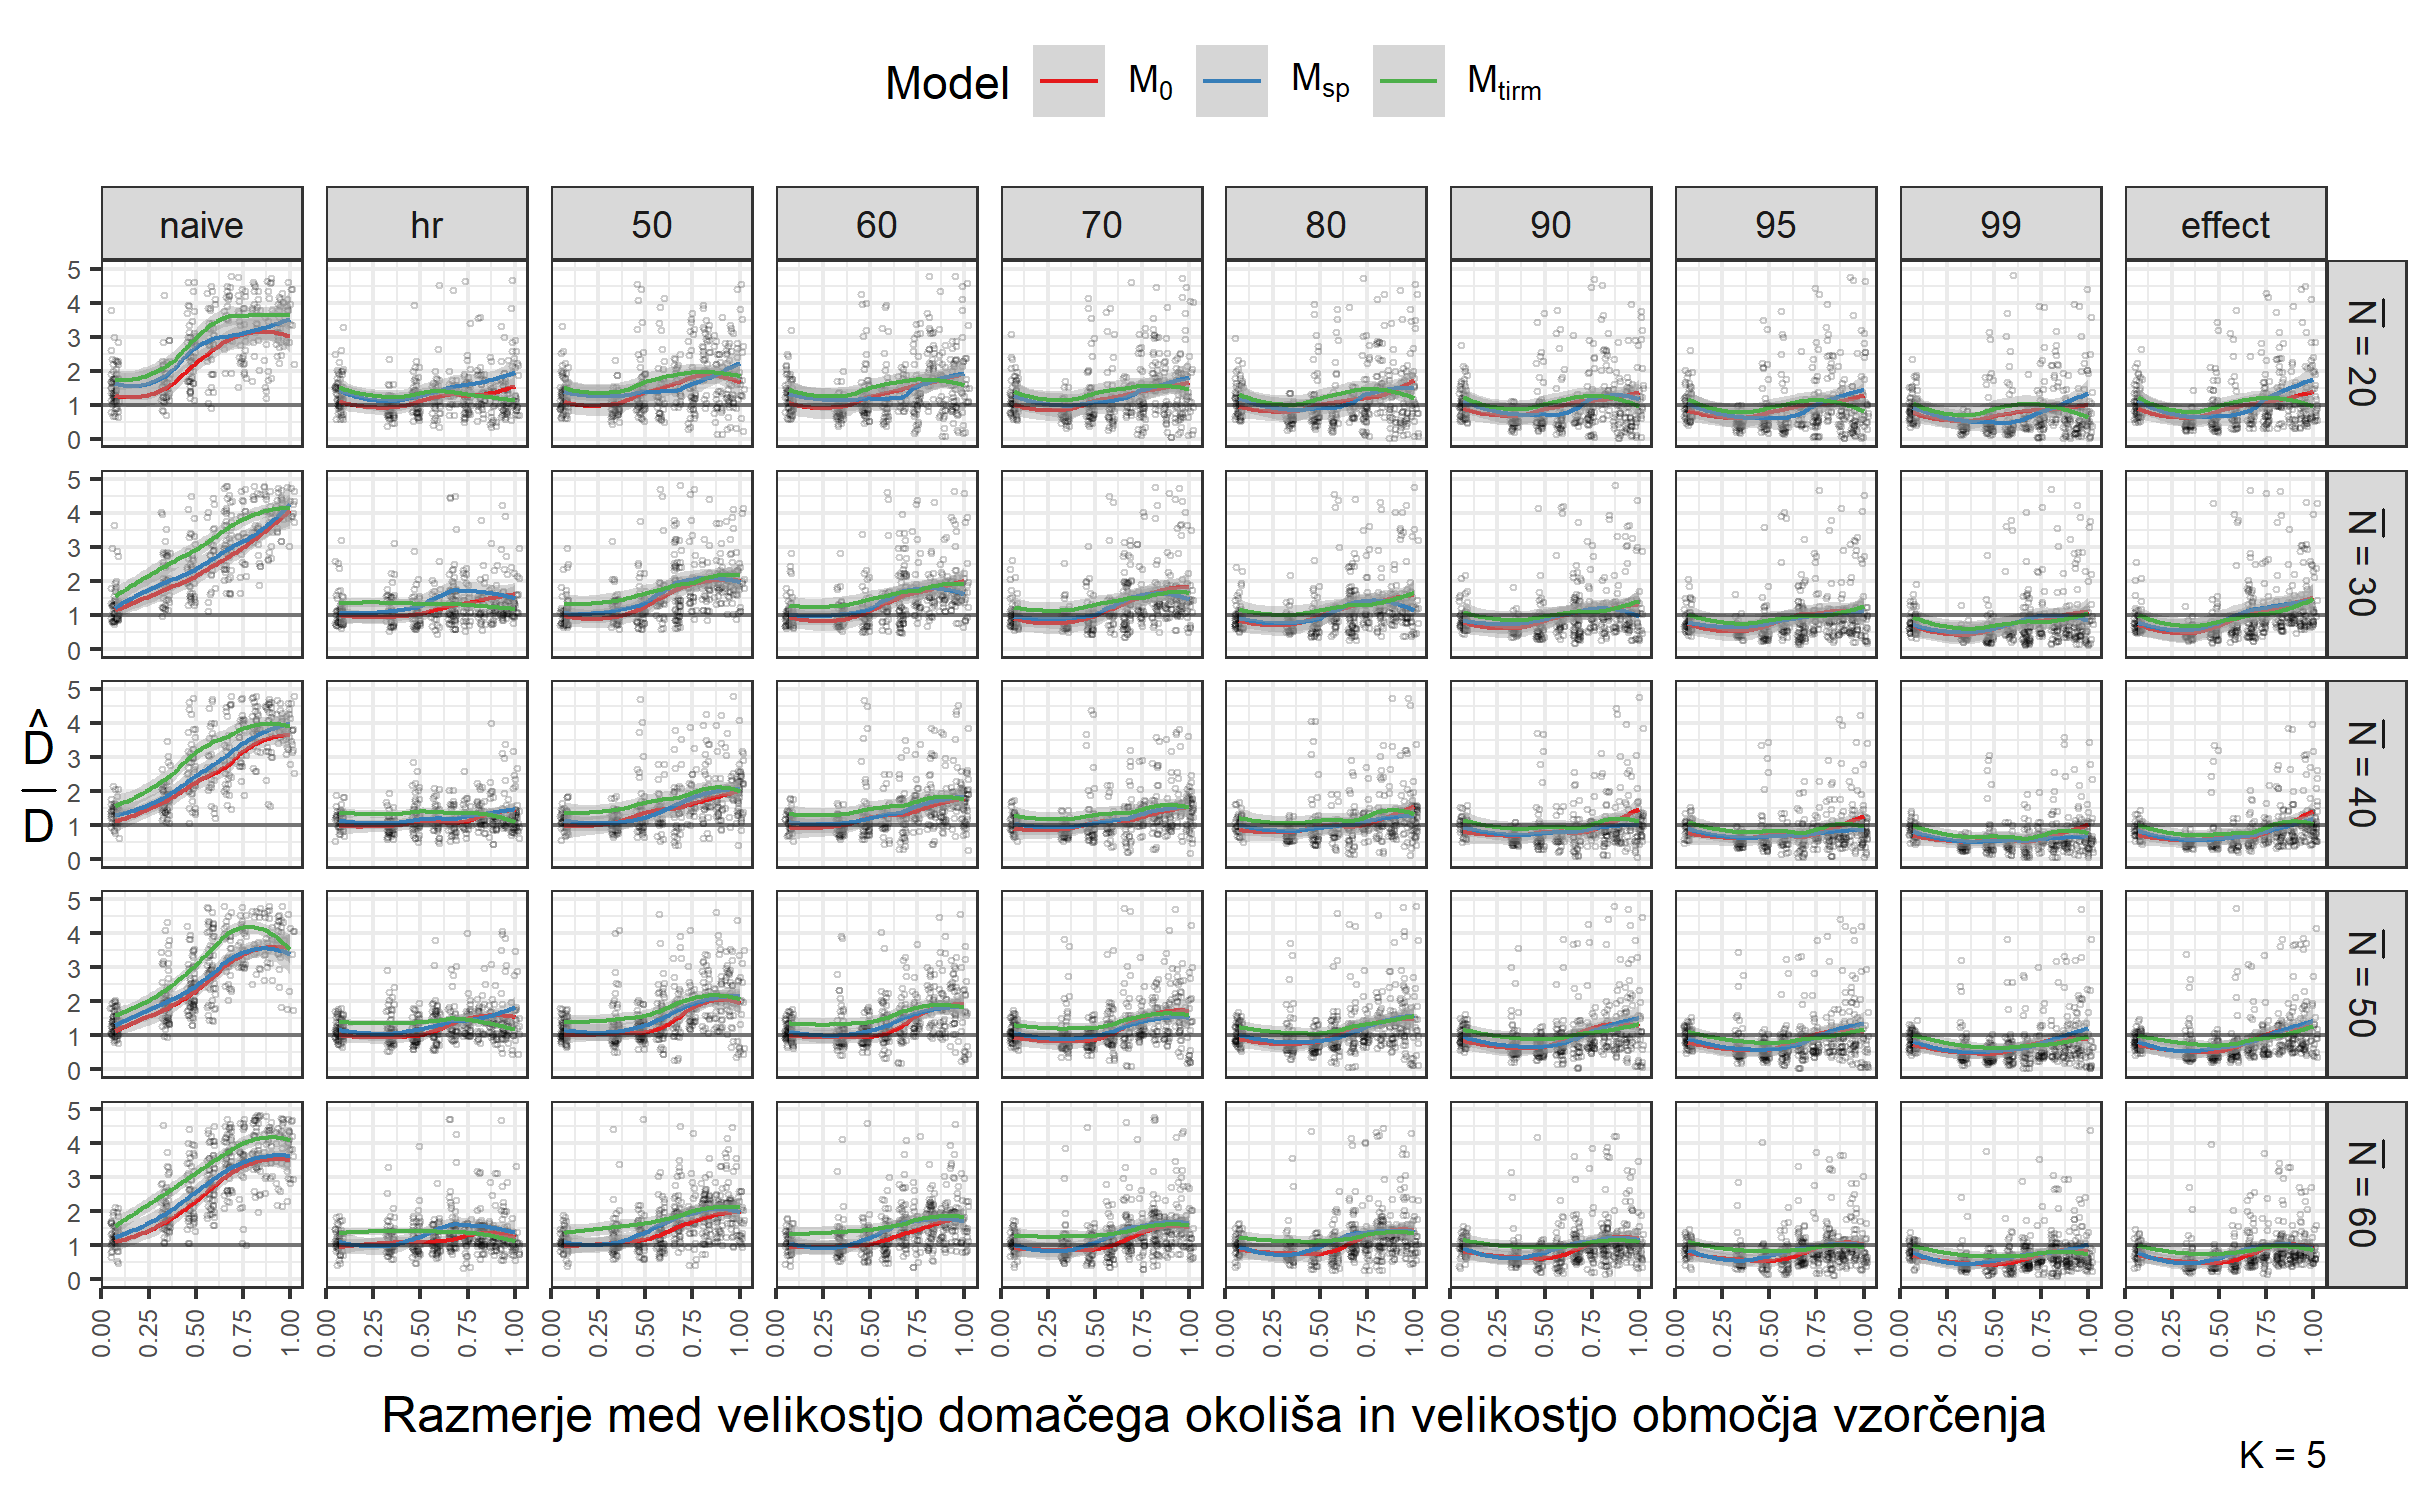
\includegraphics[width=1\linewidth]{C:/Users/romunov/Documents/workspace/doktorat/analiza/figures/E-1c_gostota_gled_na_razmerje_hr_sap_po_correction_type_in_st_gen_walk_za_k5.png}
    \label{sli:sub8.1}
  \end{subfigure}

  \begin{subfigure}[b]{1\textwidth}
    \centering
    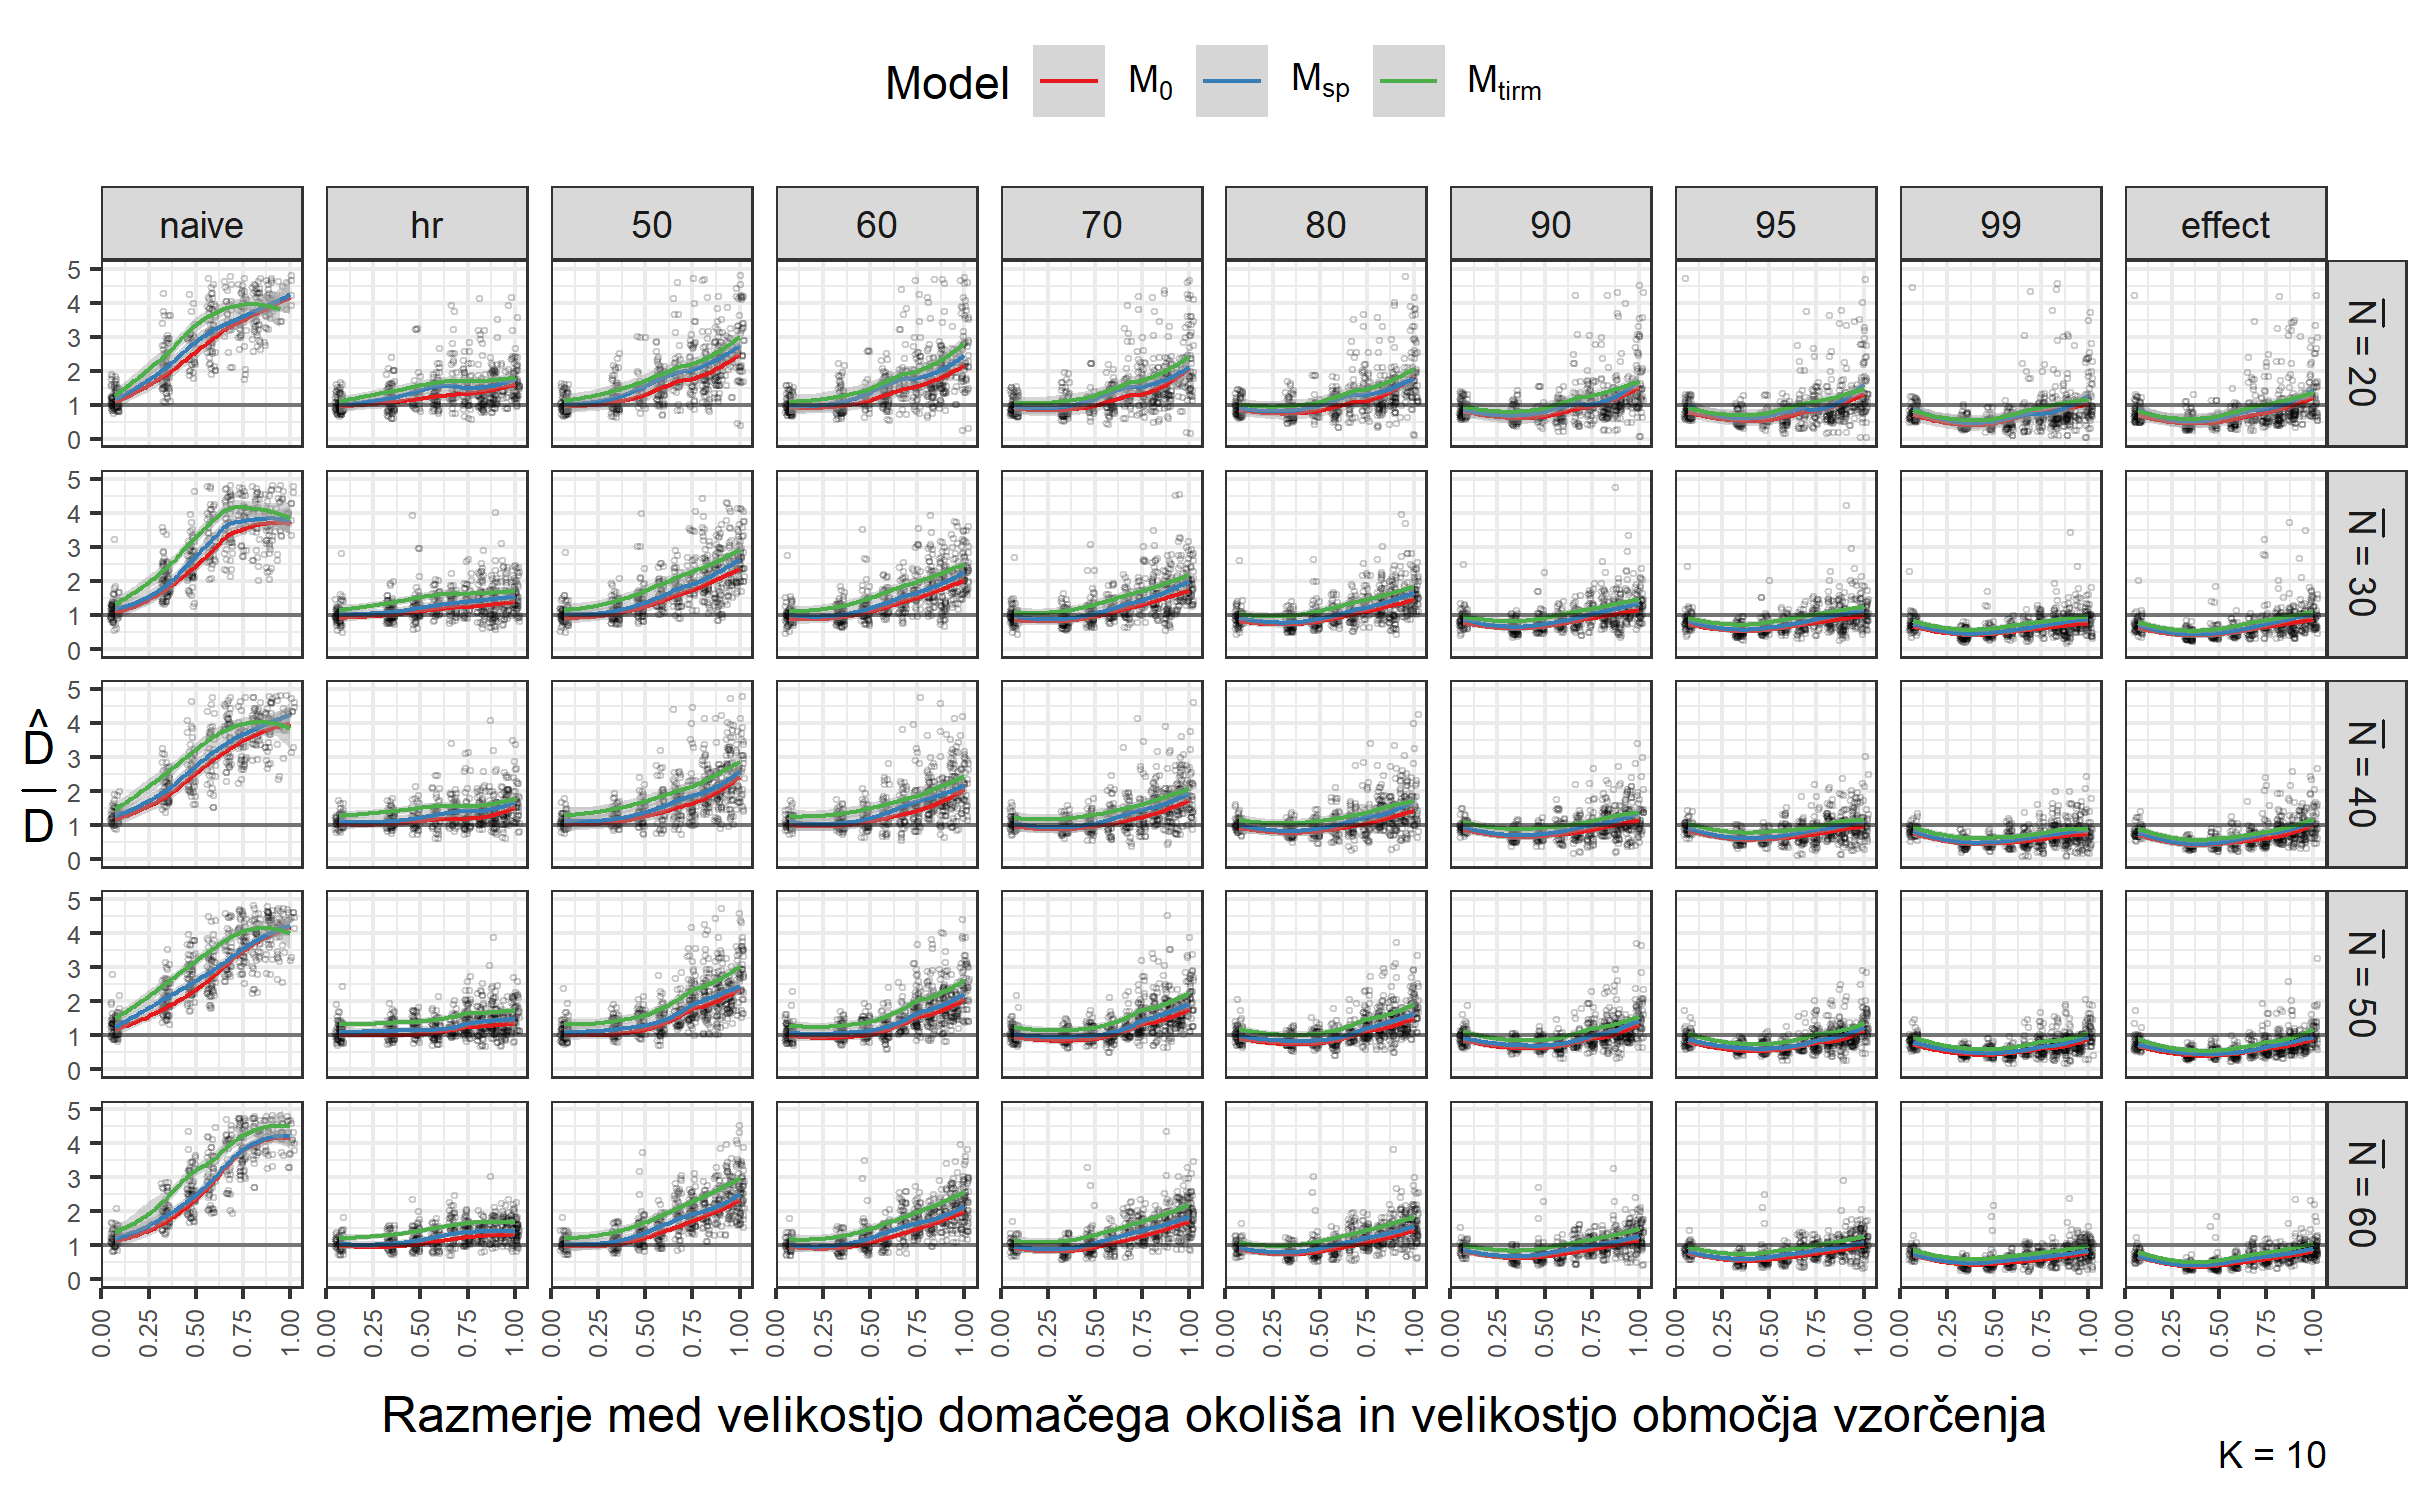
\includegraphics[width=1\linewidth]{C:/Users/romunov/Documents/workspace/doktorat/analiza/figures/E-1d_gostota_glede_na_razmerje_hr_sap_po_correction_type_in_st_gen_walk_za_k10.png}
    \label{sli:sub8.2}
  \end{subfigure}
\end{figure}

\begin{figure}[H]
  \ContinuedFloat
  \begin{subfigure}[b]{1\textwidth}
    \centering
    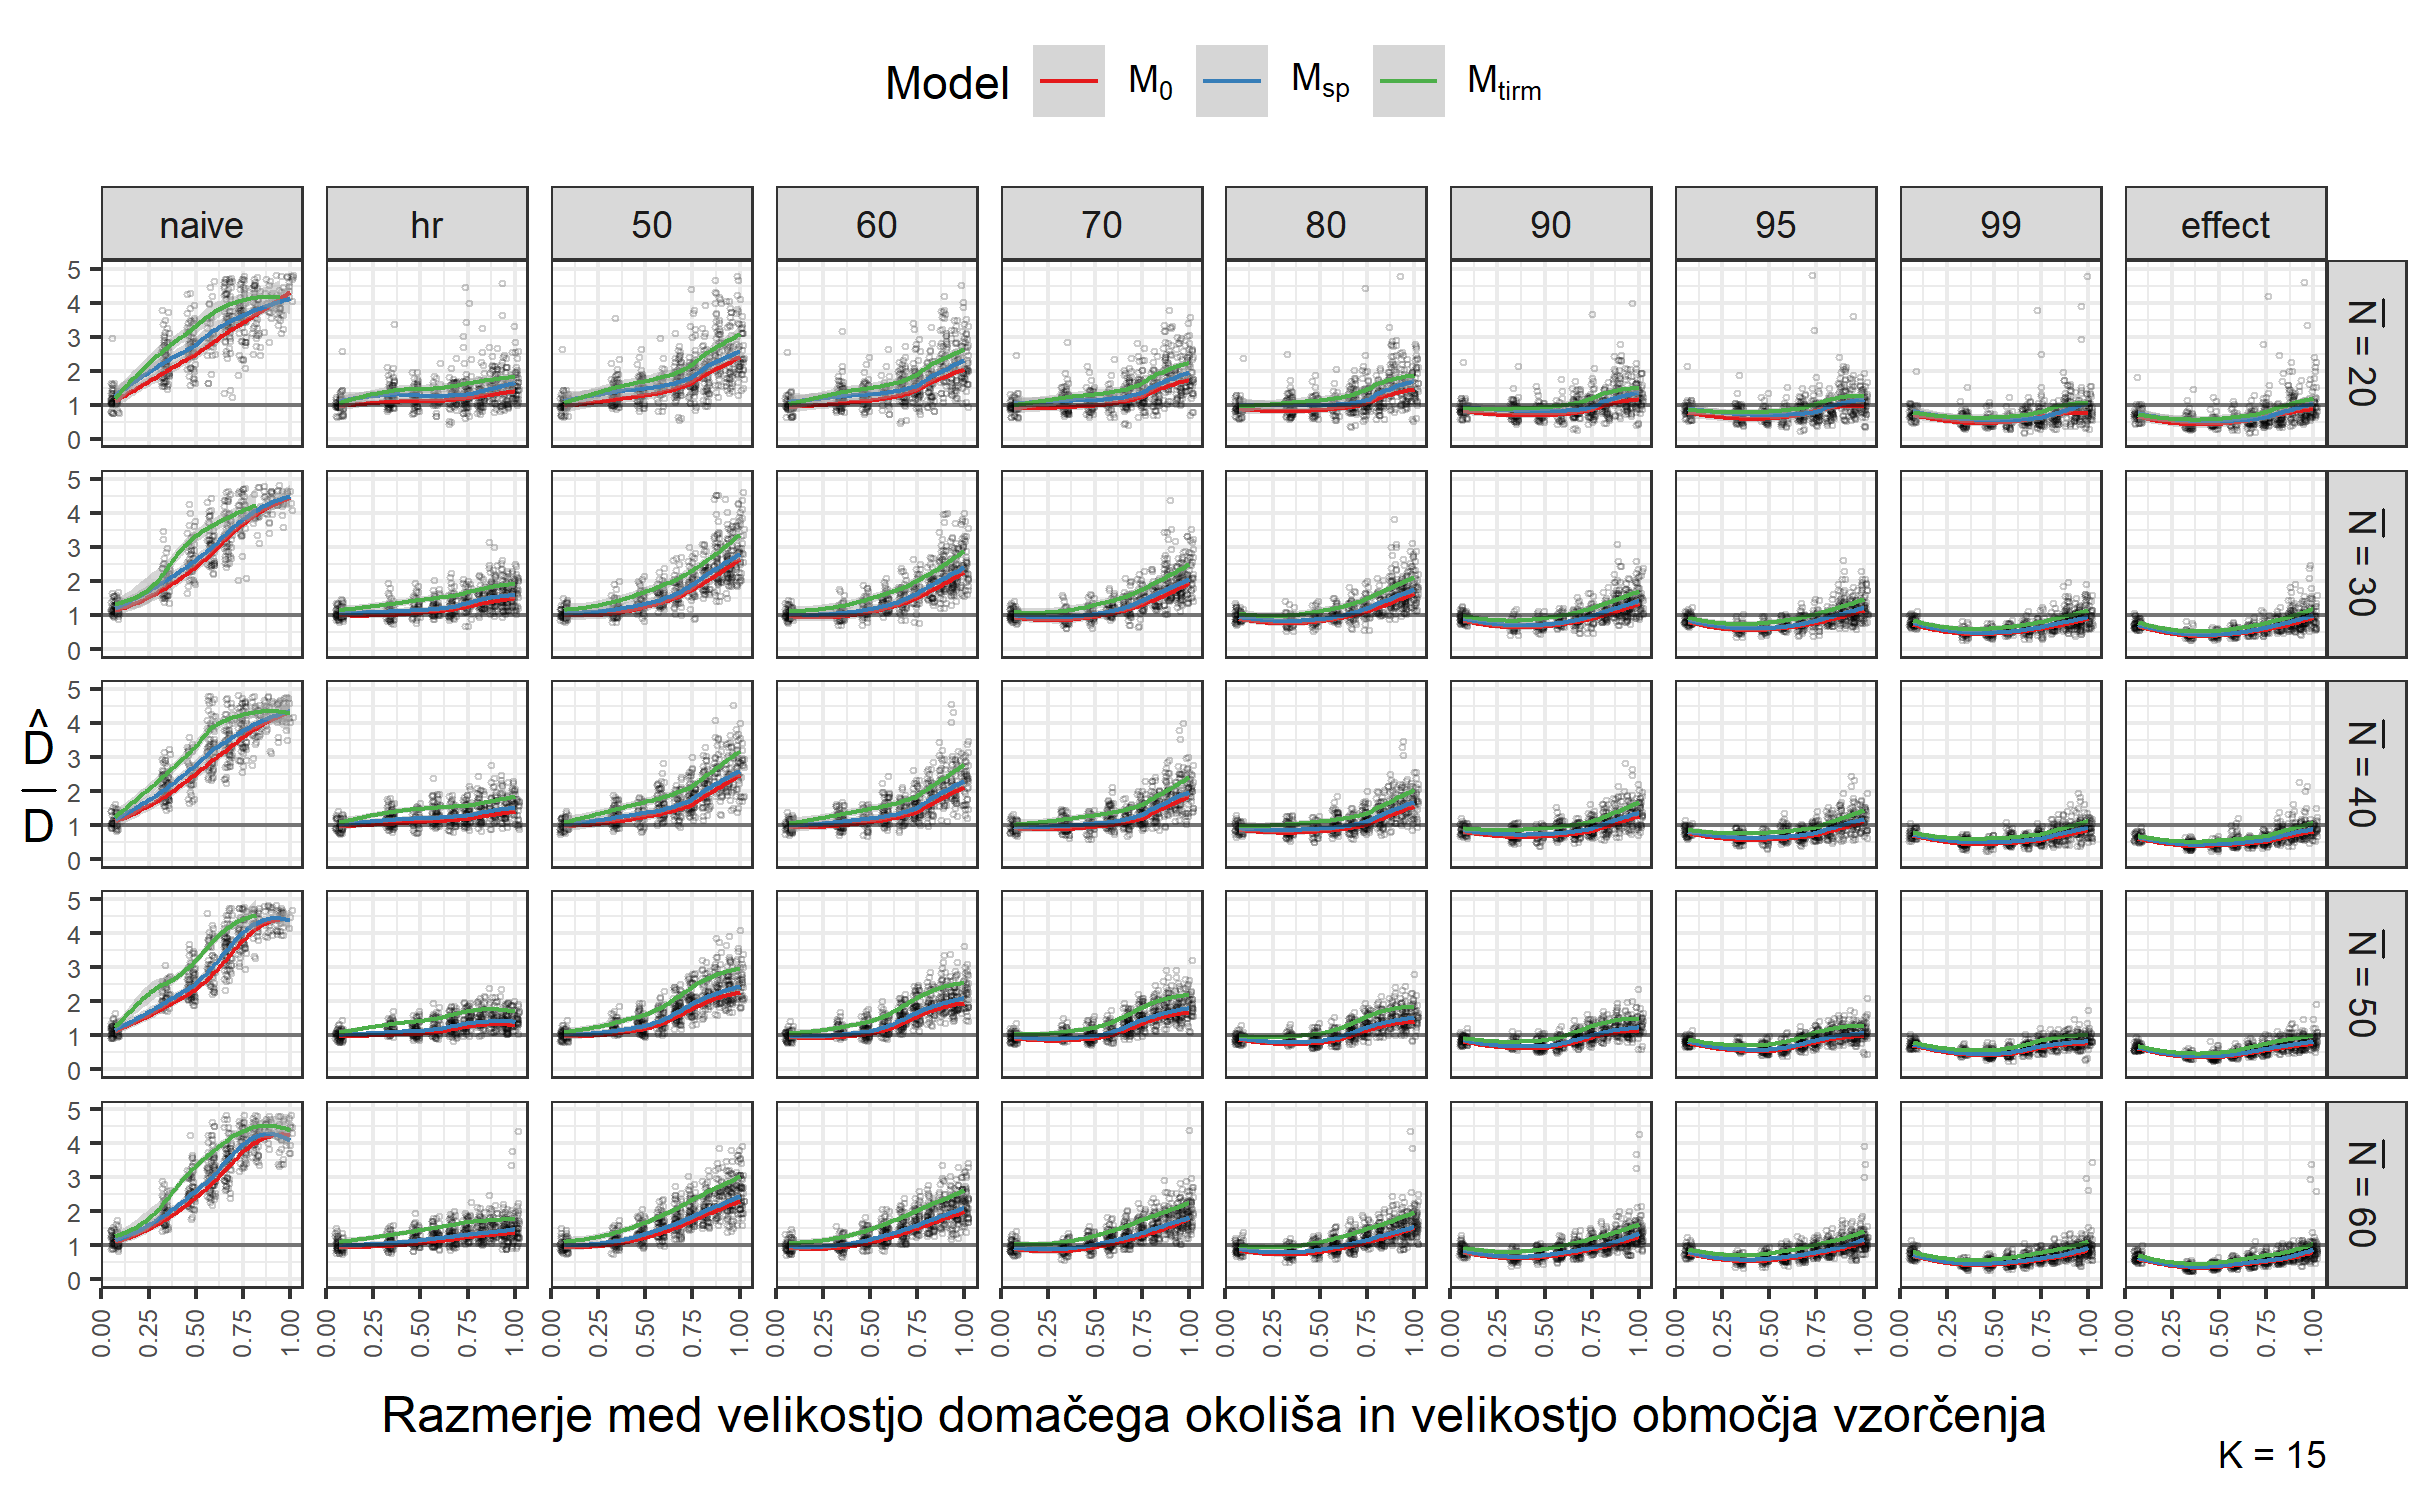
\includegraphics[width=1\linewidth]{C:/Users/romunov/Documents/workspace/doktorat/analiza/figures/E-1e_gostota_glede_na_razmerje_hr_sap_po_correction_type_in_st_gen_walk_za_k15.png}
    \label{sli:sub8.3}
  \end{subfigure}
  \caption[Prikaz ocenjene gostote (empirična porazdelitev)]{Prikaz ocenjene gostote (empirična porazdelitev). Bolj podroben prikaz podatkov s slike \ref{sli:slika7} (zgoraj, individualna spremenljivka izračunana s pomočjo empirične porazdelitve), kjer smo podatke dodatno prikazali glede na število odlovnih intervalov ($K$). Zgoraj $K=5$, v sredini $K=10$, spodaj $K=15$.

  \medskip

  Figure \ref{sli:slika8}: Depiction of estimated densities (empirical distribution). Same data as depicted in figure \ref{sli:slika7} (upper, individual covariate calculated using empirical distribution), but also sliced according to number of sampling sessions ($K=5$ above, $K=10$ in the middle and $K=15$ at the bottom).}
  \label{sli:slika8}
\end{figure}

\begin{figure}[H]
  % \ContinuedFloat
  \centering
  \begin{subfigure}[b]{1\textwidth}
    \centering
    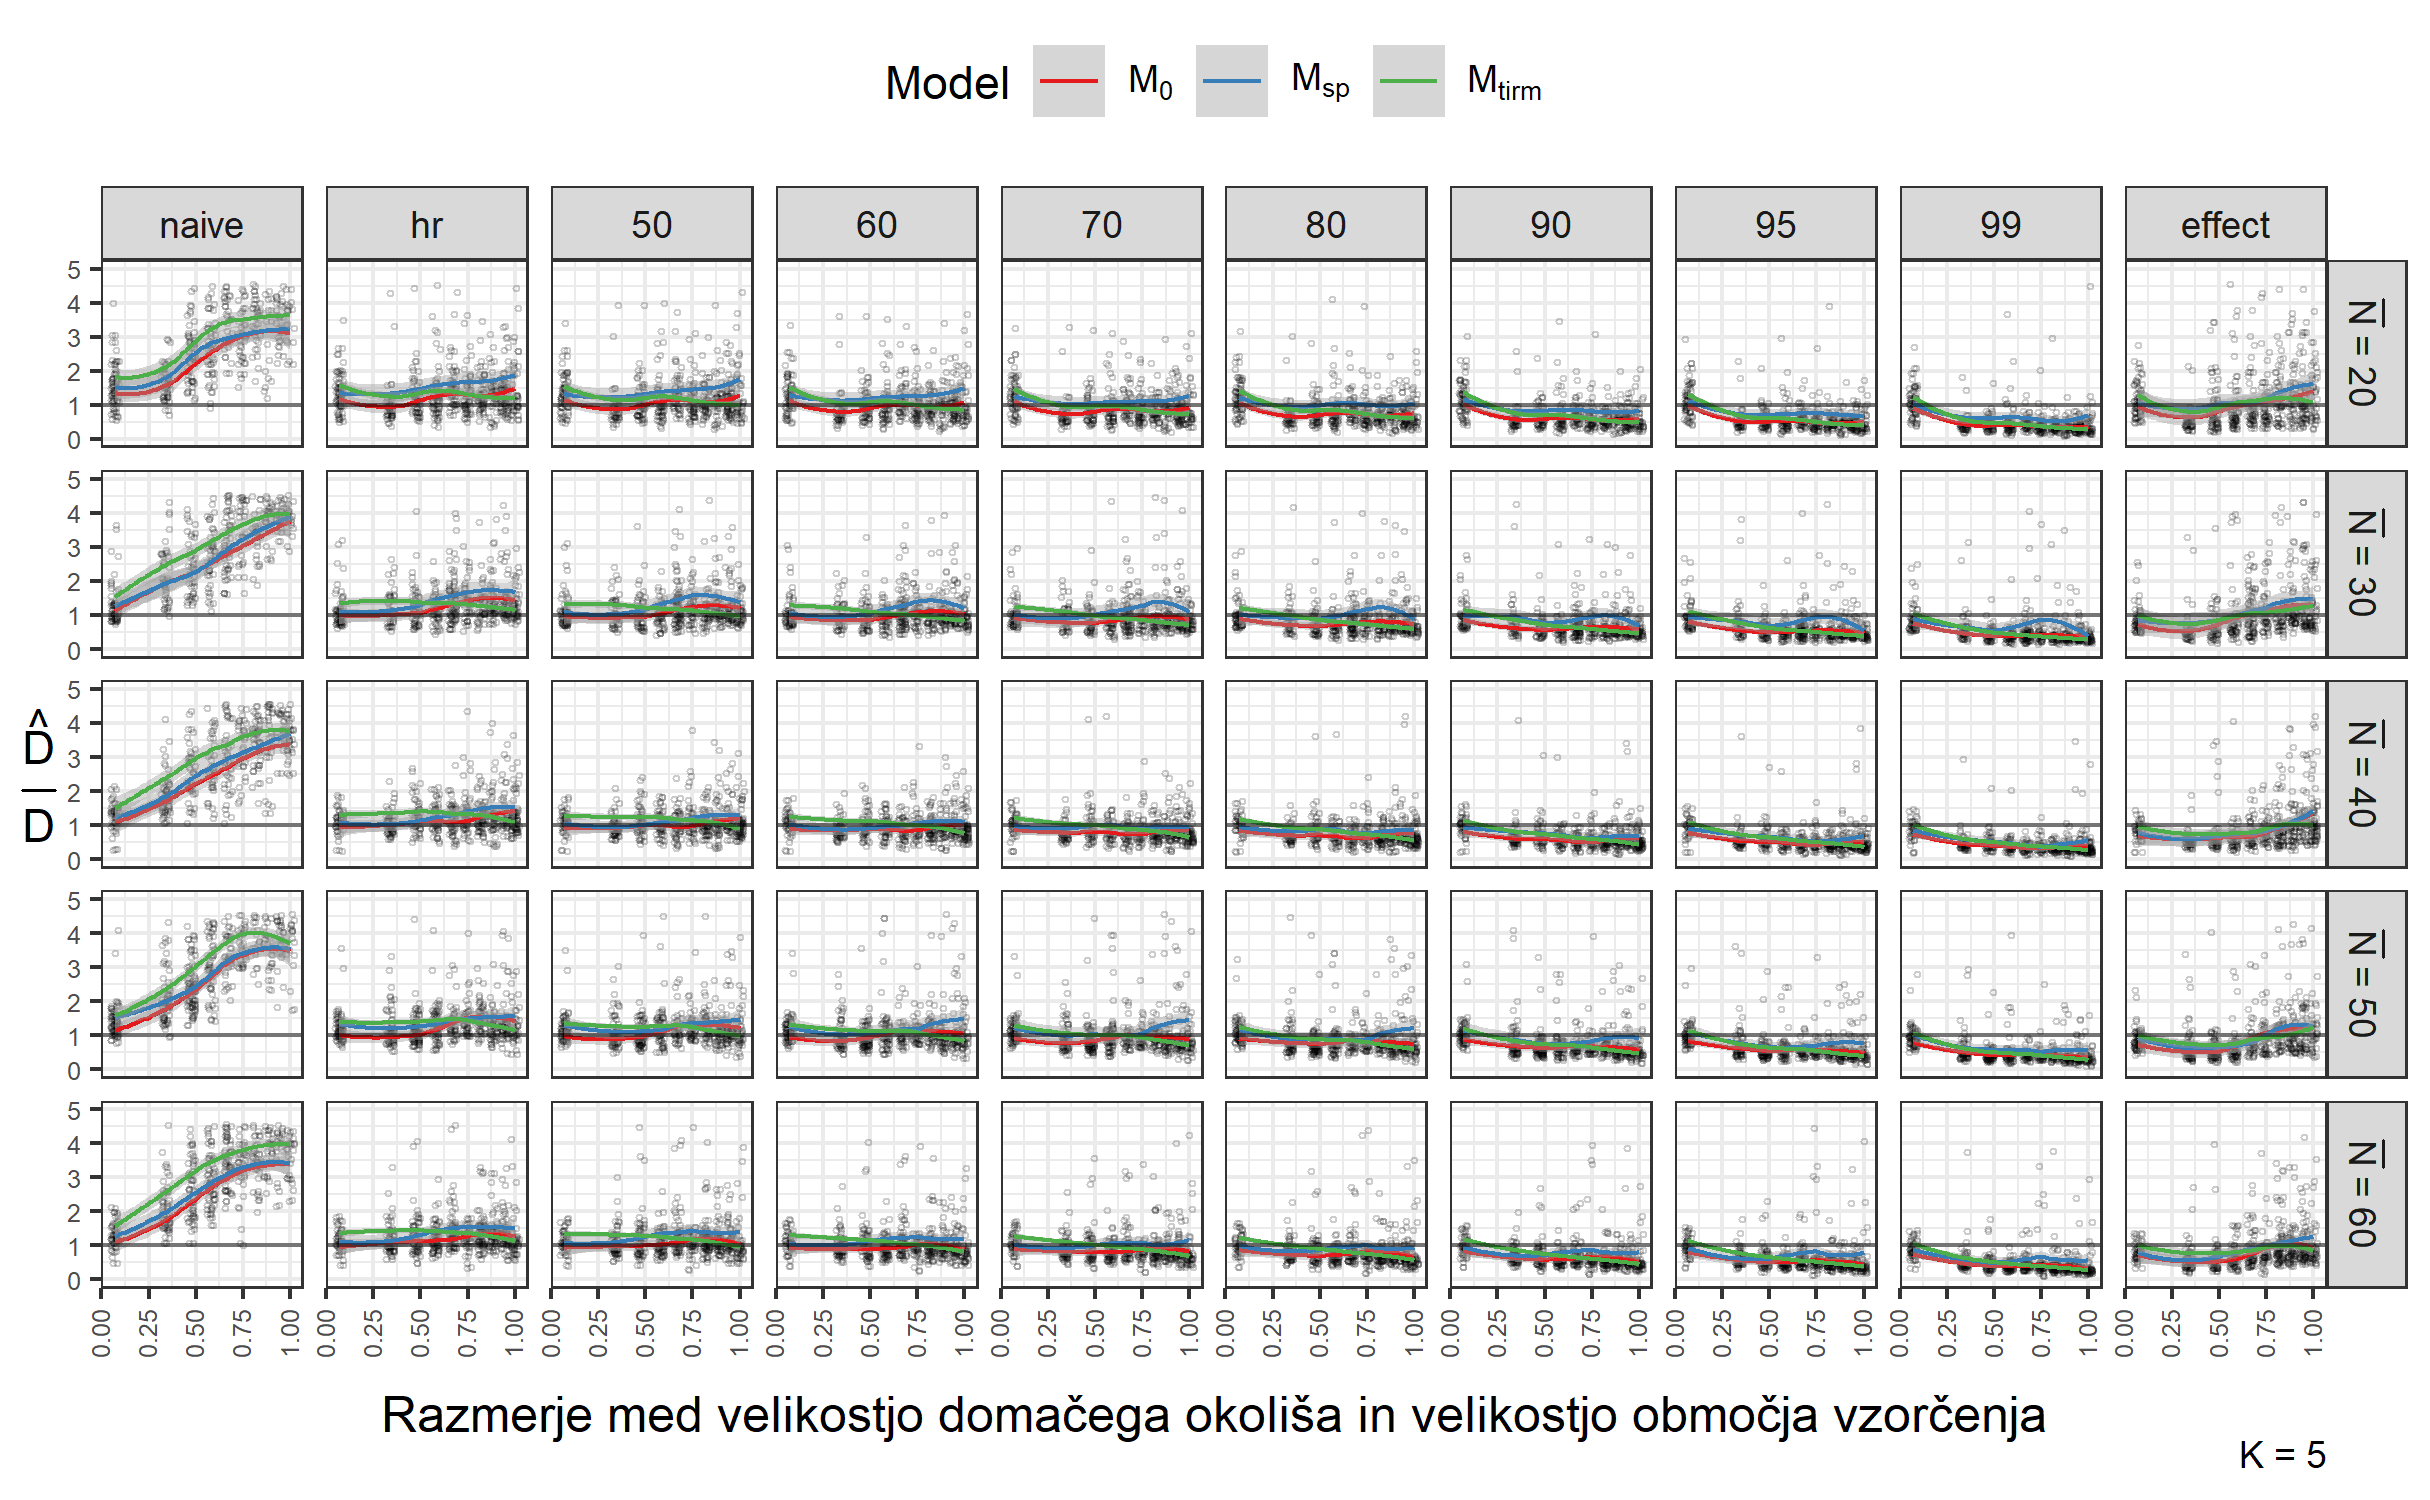
\includegraphics[width=1\linewidth]{C:/Users/romunov/Documents/workspace/doktorat/analiza/figures/N-1c_gostota_gled_na_razmerje_hr_sap_po_correction_type_in_st_gen_walk_za_k5.png}
    \label{sli:sub9.1}
  \end{subfigure}

  \begin{subfigure}[b]{1\textwidth}
    \centering
    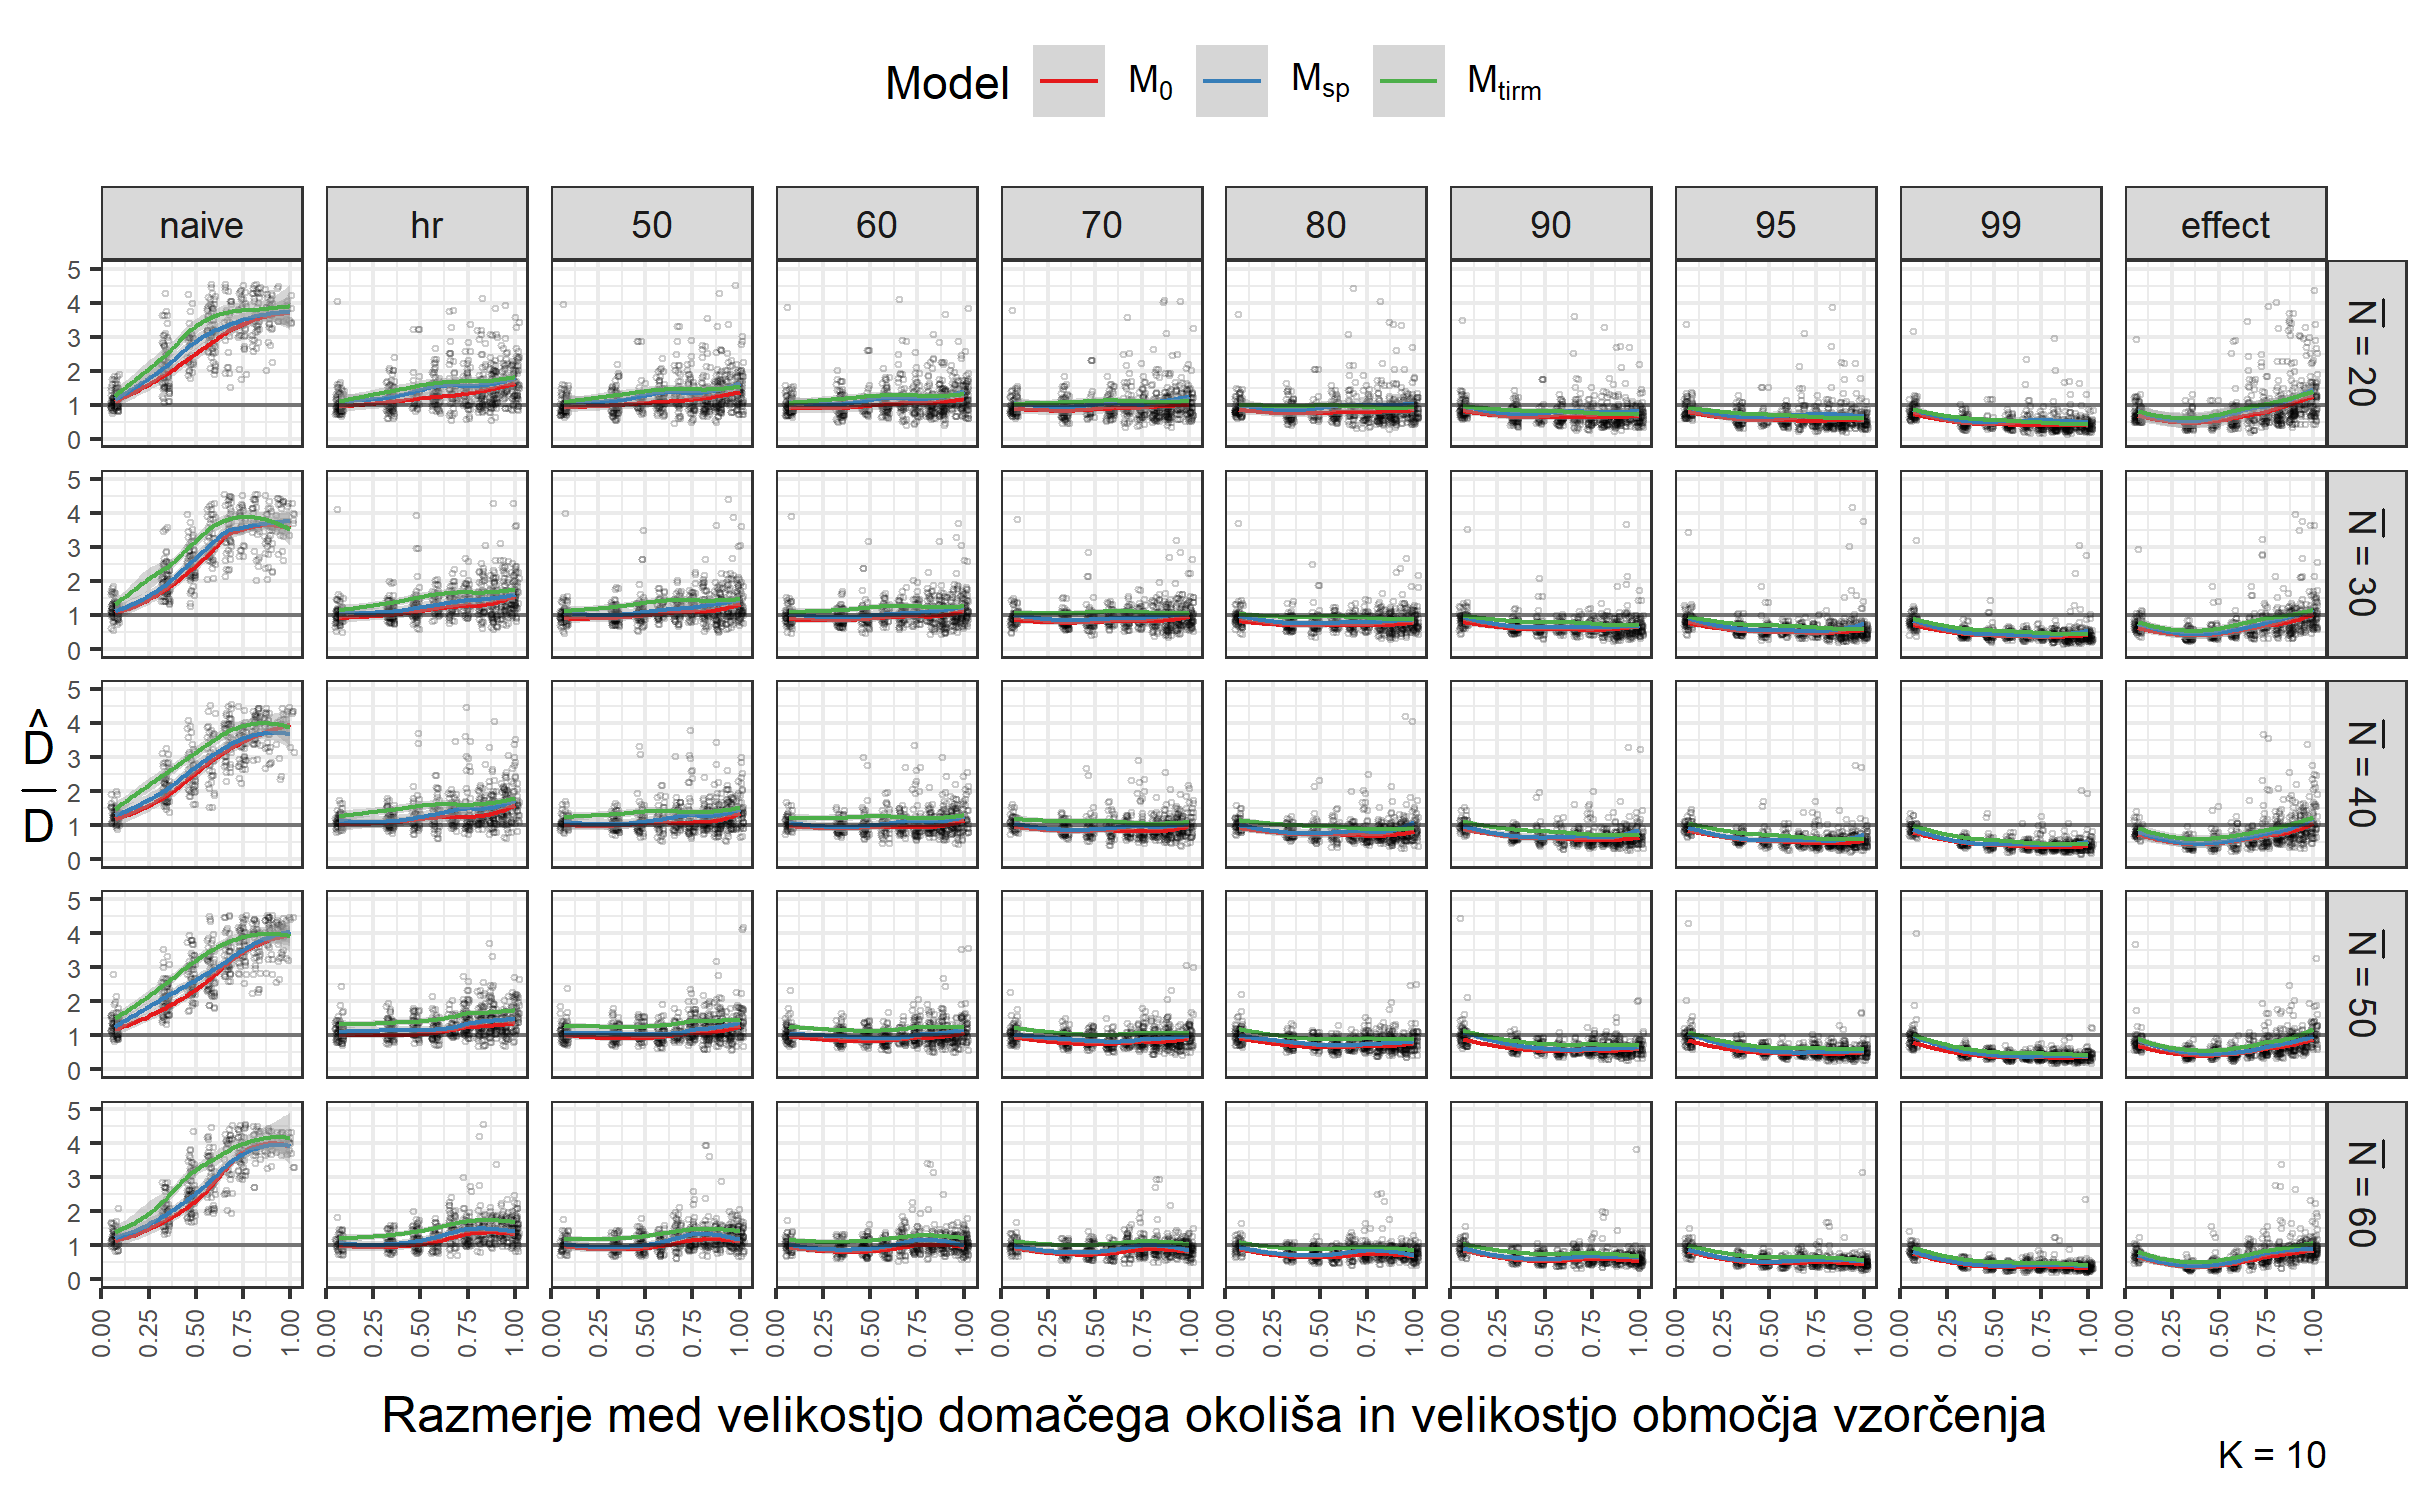
\includegraphics[width=1\linewidth]{C:/Users/romunov/Documents/workspace/doktorat/analiza/figures/N-1d_gostota_glede_na_razmerje_hr_sap_po_correction_type_in_st_gen_walk_za_k10.png}
    \label{sli:sub9.2}
  \end{subfigure}
\end{figure}

\begin{figure}[H]
  \ContinuedFloat
  \begin{subfigure}[b]{1\textwidth}
    \centering
    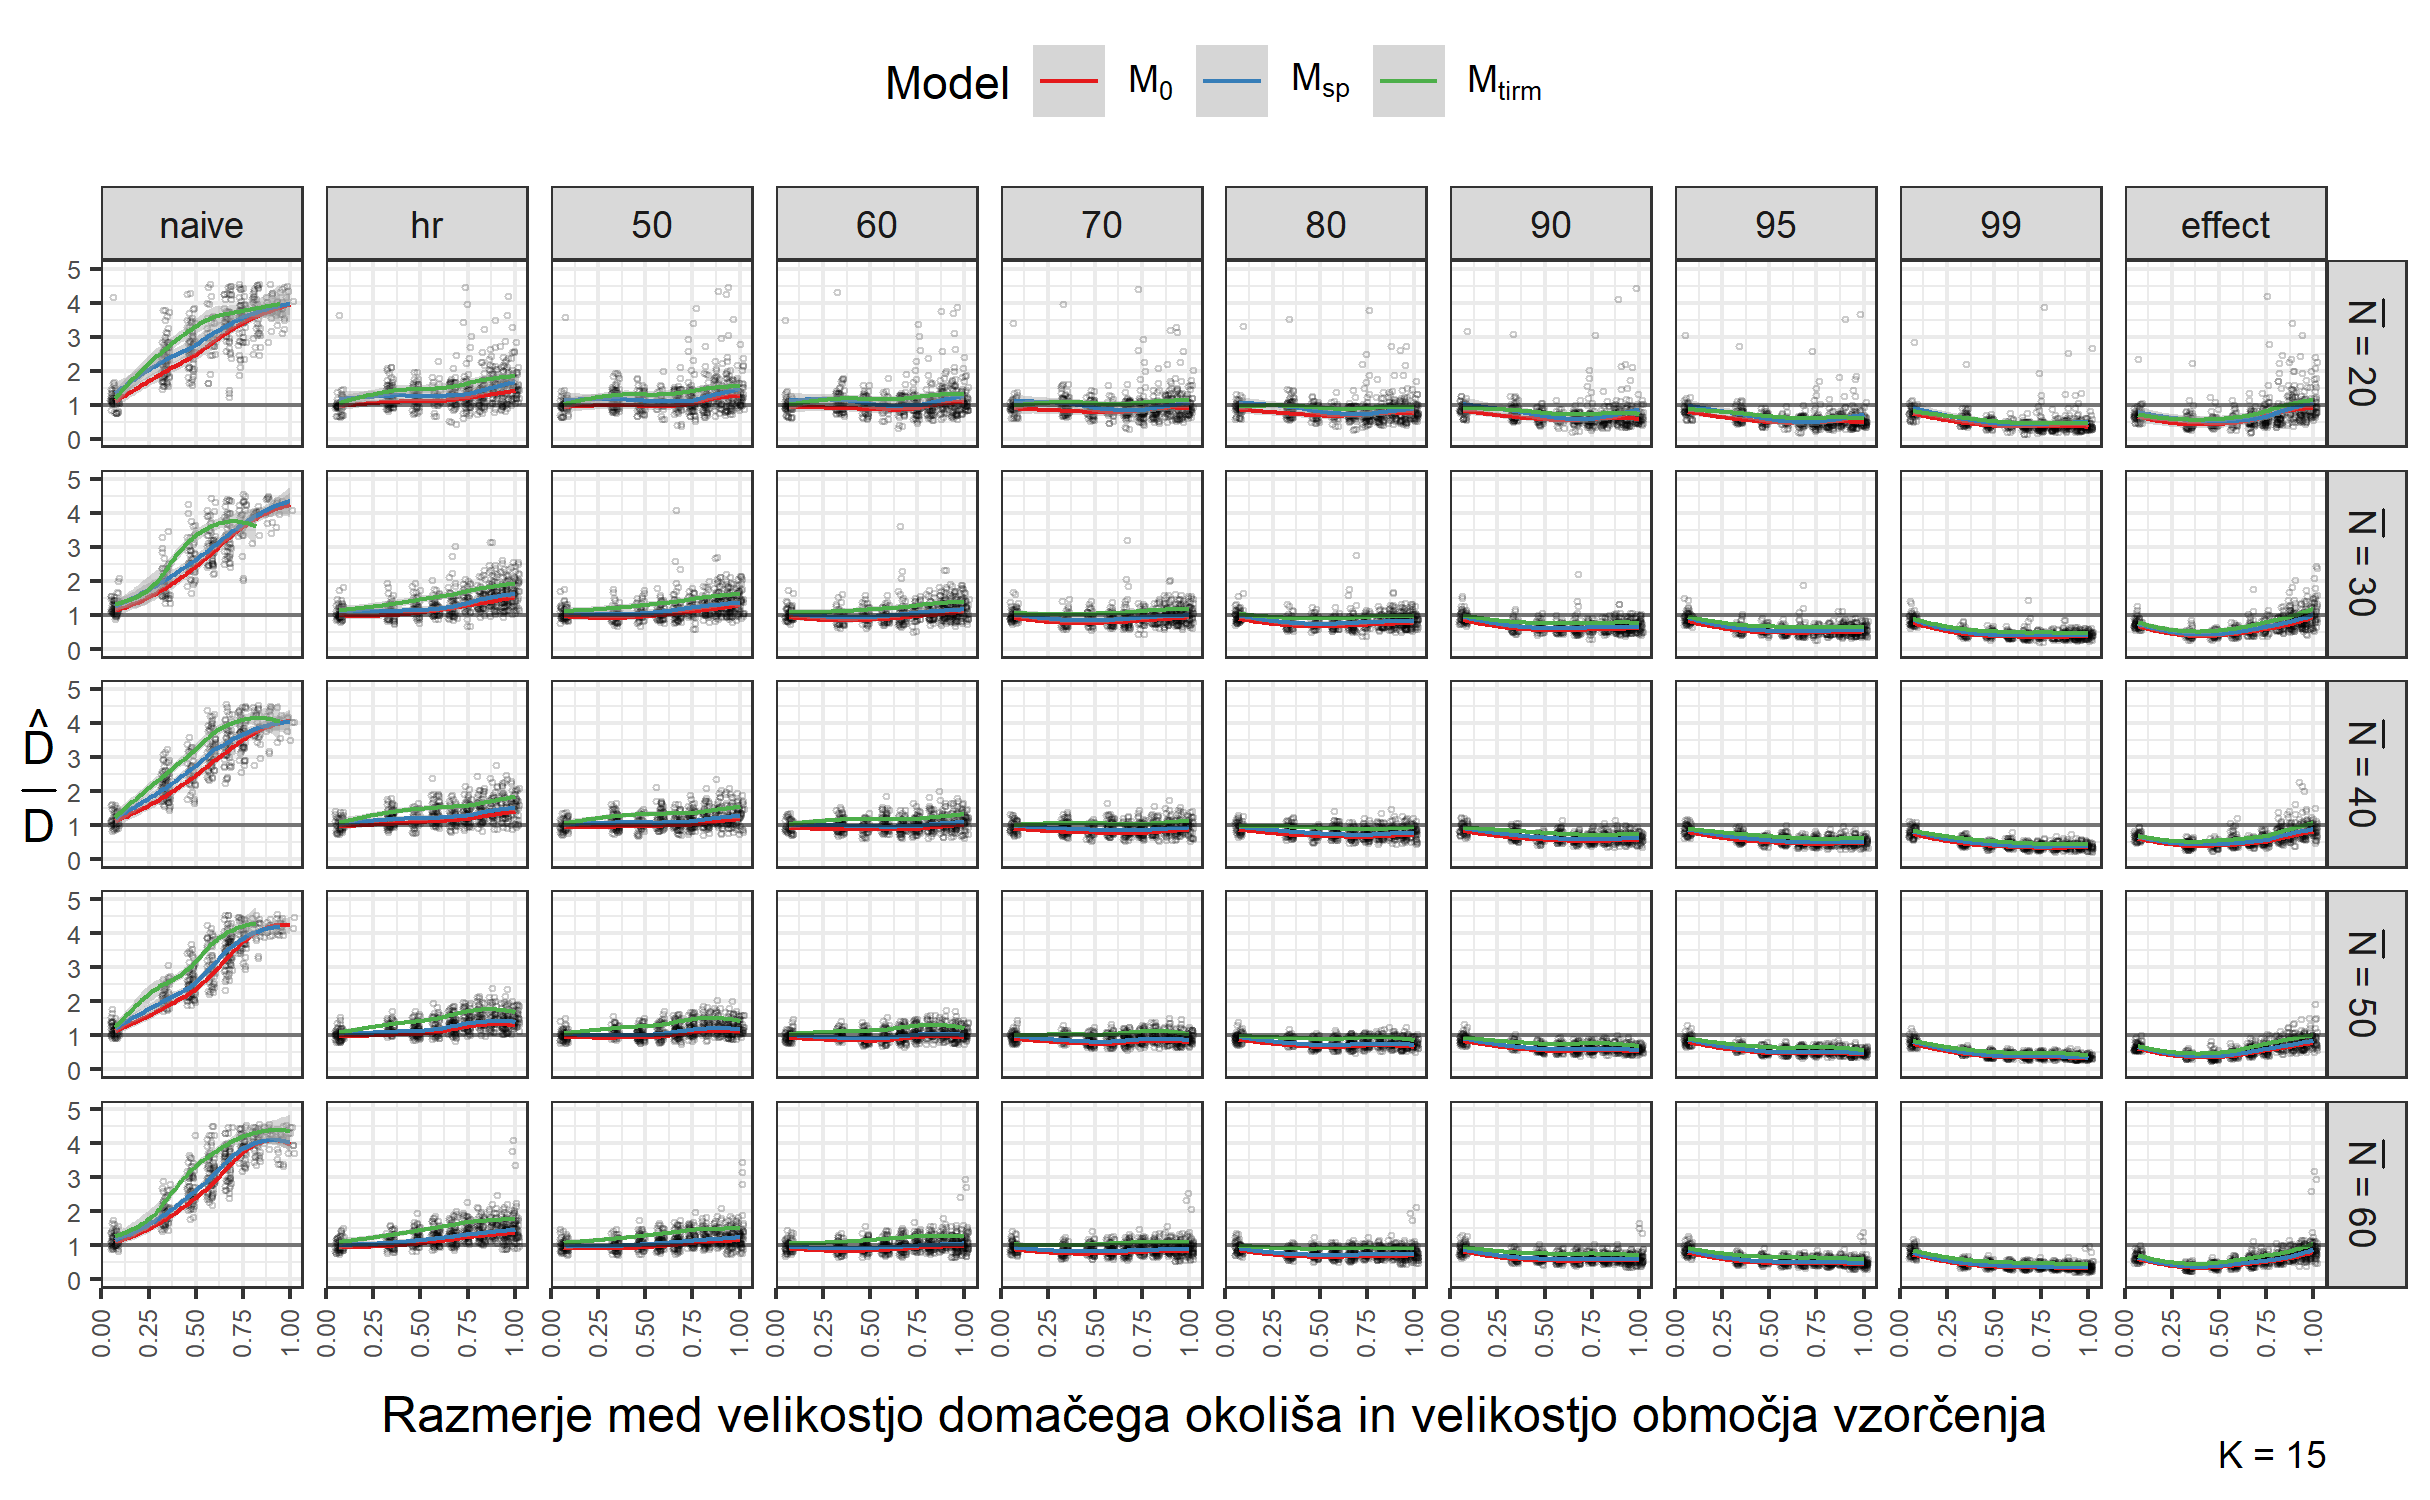
\includegraphics[width=1\linewidth]{C:/Users/romunov/Documents/workspace/doktorat/analiza/figures/N-1e_gostota_glede_na_razmerje_hr_sap_po_correction_type_in_st_gen_walk_za_k15.png}
    \label{sli:sub9.3}
  \end{subfigure}
  \caption[Prikaz ocenjene gostote (normalna porazdelitev)]{Prikaz ocenjene gostote (normalna porazdelitev). Bolj podroben prikaz podatkov s slike \ref{sli:slika7} (spodaj, individualna spremenljivka izračunana s pomočjo dvorazsežne normalne porazdelitve), kjer smo podatke dodatno prikazali glede na število odlovnih intervalov ($K$). Zgoraj $K=5$, v sredini $K=10$, spodaj $K=15$.

  \medskip

  Figure \ref{sli:slika9}: Depiction of estimated densities (normal distribution). Same data as depicted in figure \ref{sli:slika7} (lower, individual covariate calculated using two-dimensional normal distribution), but also sliced according to number of sampling sessions ($K=5$ above, $K=10$ in the middle and $K=15$ at the bottom).}
  \label{sli:slika9}
\end{figure}

\subsection{AICc}
Metriko AICc smo primerjali samo za Hugginsova modela $M_0$ in $M_{sp}$. Verjetje modela TIRM ni primerljivo s Hugginsovim modelom. Poleg druge funkcije največjega verjetja uporabi za izračun velikosti populacije drugačen set podatkov. Primerjava vrednosti AICc z ostalima dvema modeloma zato ne bi bila pravilna.

Za vsako simulacijo smo določili, kateri model ima manjši AICc, nato pa razliko med modeloma prikazali na osi $y$. Vedno smo odšteli AICc modela $M_0$ od AICc modela $M_{sp}$. Negativne vrednosti so povezane s tistimi simulacijami, kjer je bil boljši model $M_0$, pozitivne pa s simulacijami, kjer je bil boljši model $M_{sp}$. Če je bil boljši model $M_{sp}$, je bila razlika pogosto mnogo večja (modra barva) kot v primerih, ko je bil boljši model $M_0$ (rdeča barva). Število simuliranih osebkov ne vpliva na razliko v AICc, zato smo podatke prikazali brez te spremenljivke na sliki \ref{sli:slika10}.

\begin{figure}[H]
  \centering
  \begin{subfigure}[b]{1\textwidth}
    \centering
    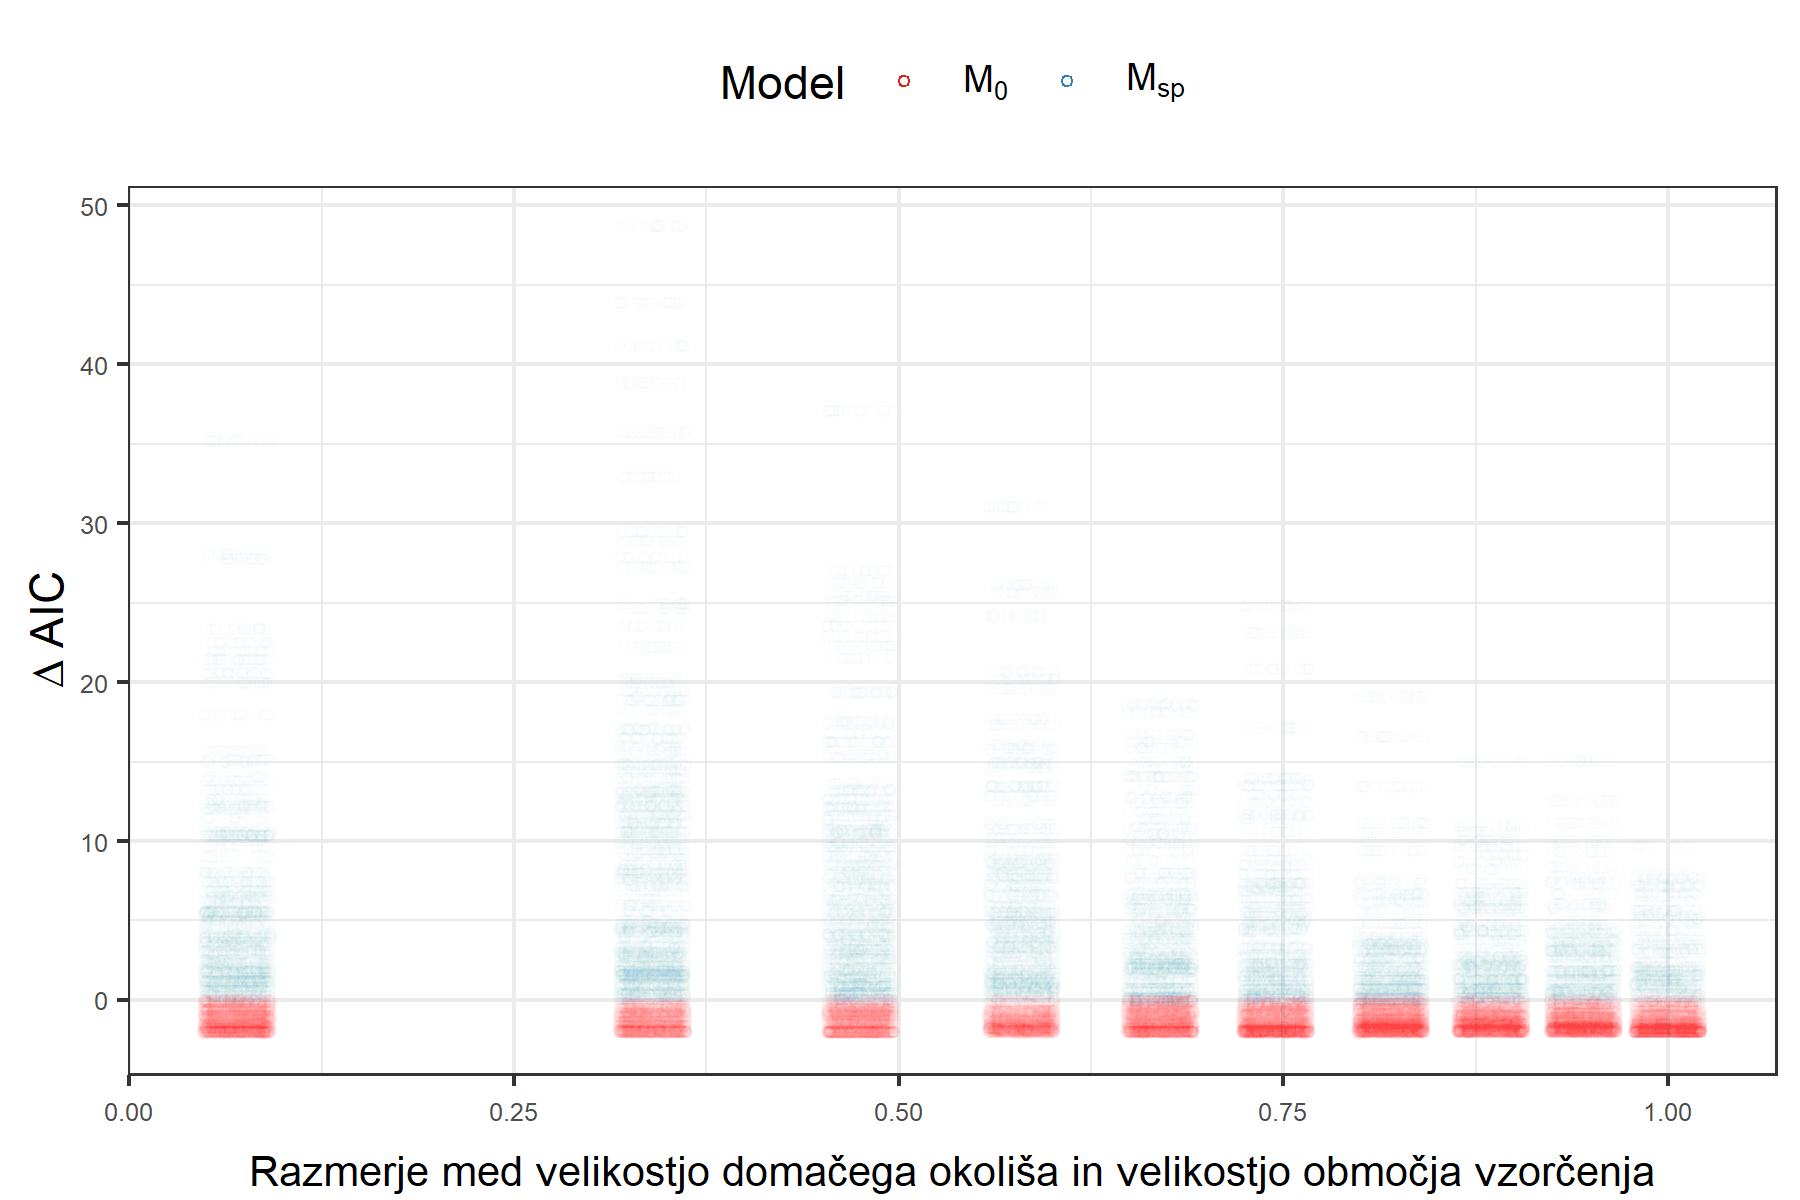
\includegraphics[width=0.9\linewidth]{C:/Users/romunov/Documents/workspace/doktorat/analiza/figures/E-6b_dAIC_glede_na_razmerje_hr_sap_po_correction_type_in_st_gen_walk_in_boljsi_model.png}
    \label{sli:sub10.1}
  \end{subfigure}

  \begin{subfigure}[b]{1\textwidth}
    \centering
    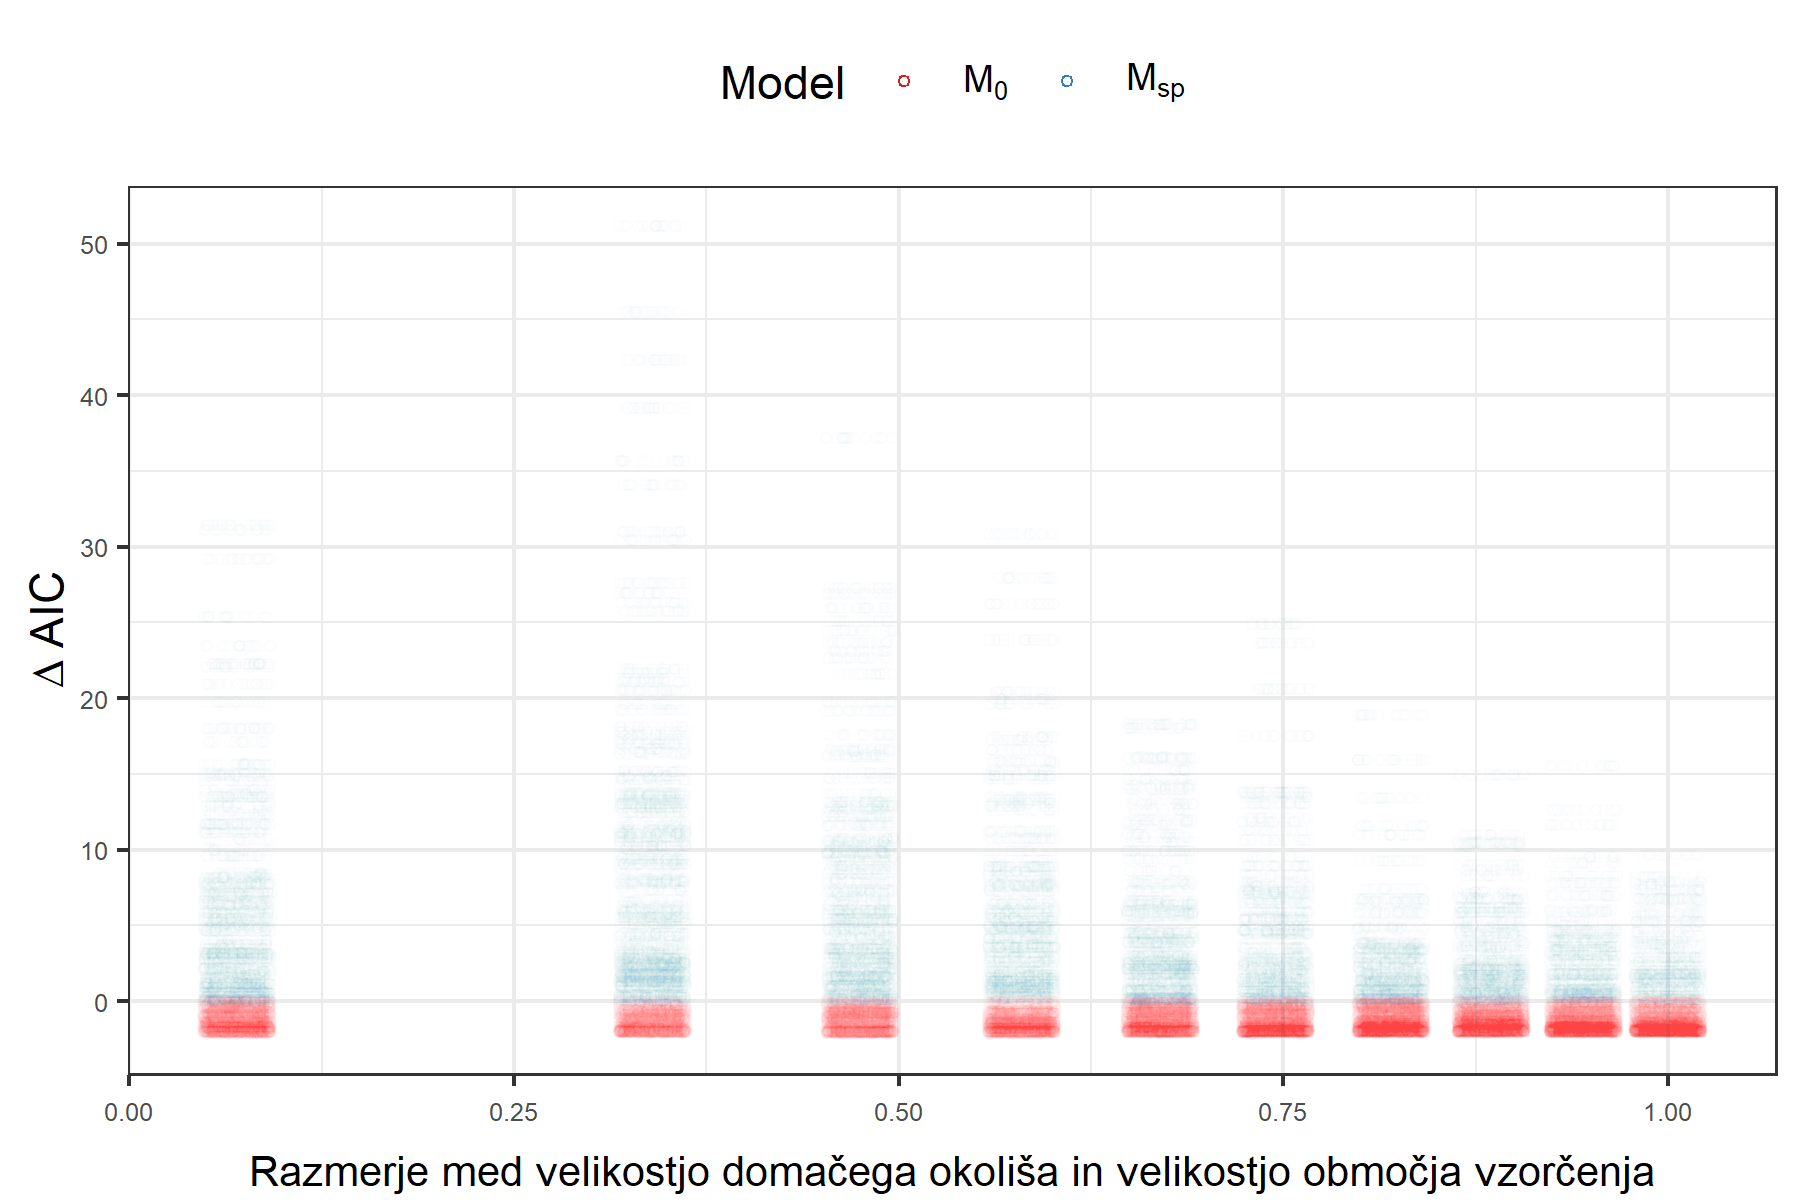
\includegraphics[width=0.9\linewidth]{C:/Users/romunov/Documents/workspace/doktorat/analiza/figures/N-6b_dAIC_glede_na_razmerje_hr_sap_po_correction_type_in_st_gen_walk_in_boljsi_model.png}
    \label{sli:sub10.2}
  \end{subfigure}
  \caption[Prikaz razlike v AICc za modela $M_0$ in $M_{sp}$]{Prikaz razlike v AICc za modela $M_0$ in $M_{sp}$. Na zgornji sliki so prikazani podatki, kjer smo za izračun individualne spremenljivke uporabili empirično porazdelitev, na spodnji pa za normalno porazdelitev. Rdeče obarvane točke predstavljajo simulacije, kjer je bil boljši model $M_0$, v modrih pa je bil boljši $M_{sp}$.

  \medskip

  Figure \ref{sli:slika10}: Distribution of AICc for models $M_0$ and $M_{sp}$ given ratio of home range size and sampling polygon size. Upper and lower figures show data for simulations where individual covariate has been calculated using empirical and two-dimensional normal distribution, respectively. Red color depicts values where model $M_0$ was superior to model $M_{sp}$ and blue represents cases where model $M_{sp}$ was superior.}
  \label{sli:slika10}
\end{figure}

Porazdelitve vrednosti so nekoliko bolj razvidne s slike \ref{sli:slika11}. Opazimo, da glede na to, katero porazdelitev uporabimo za izračun individualne spremenljivke, v rezultatih ni razlik.

\begin{figure}[H]
  \centering
  \begin{subfigure}[b]{1\textwidth}
    \centering
    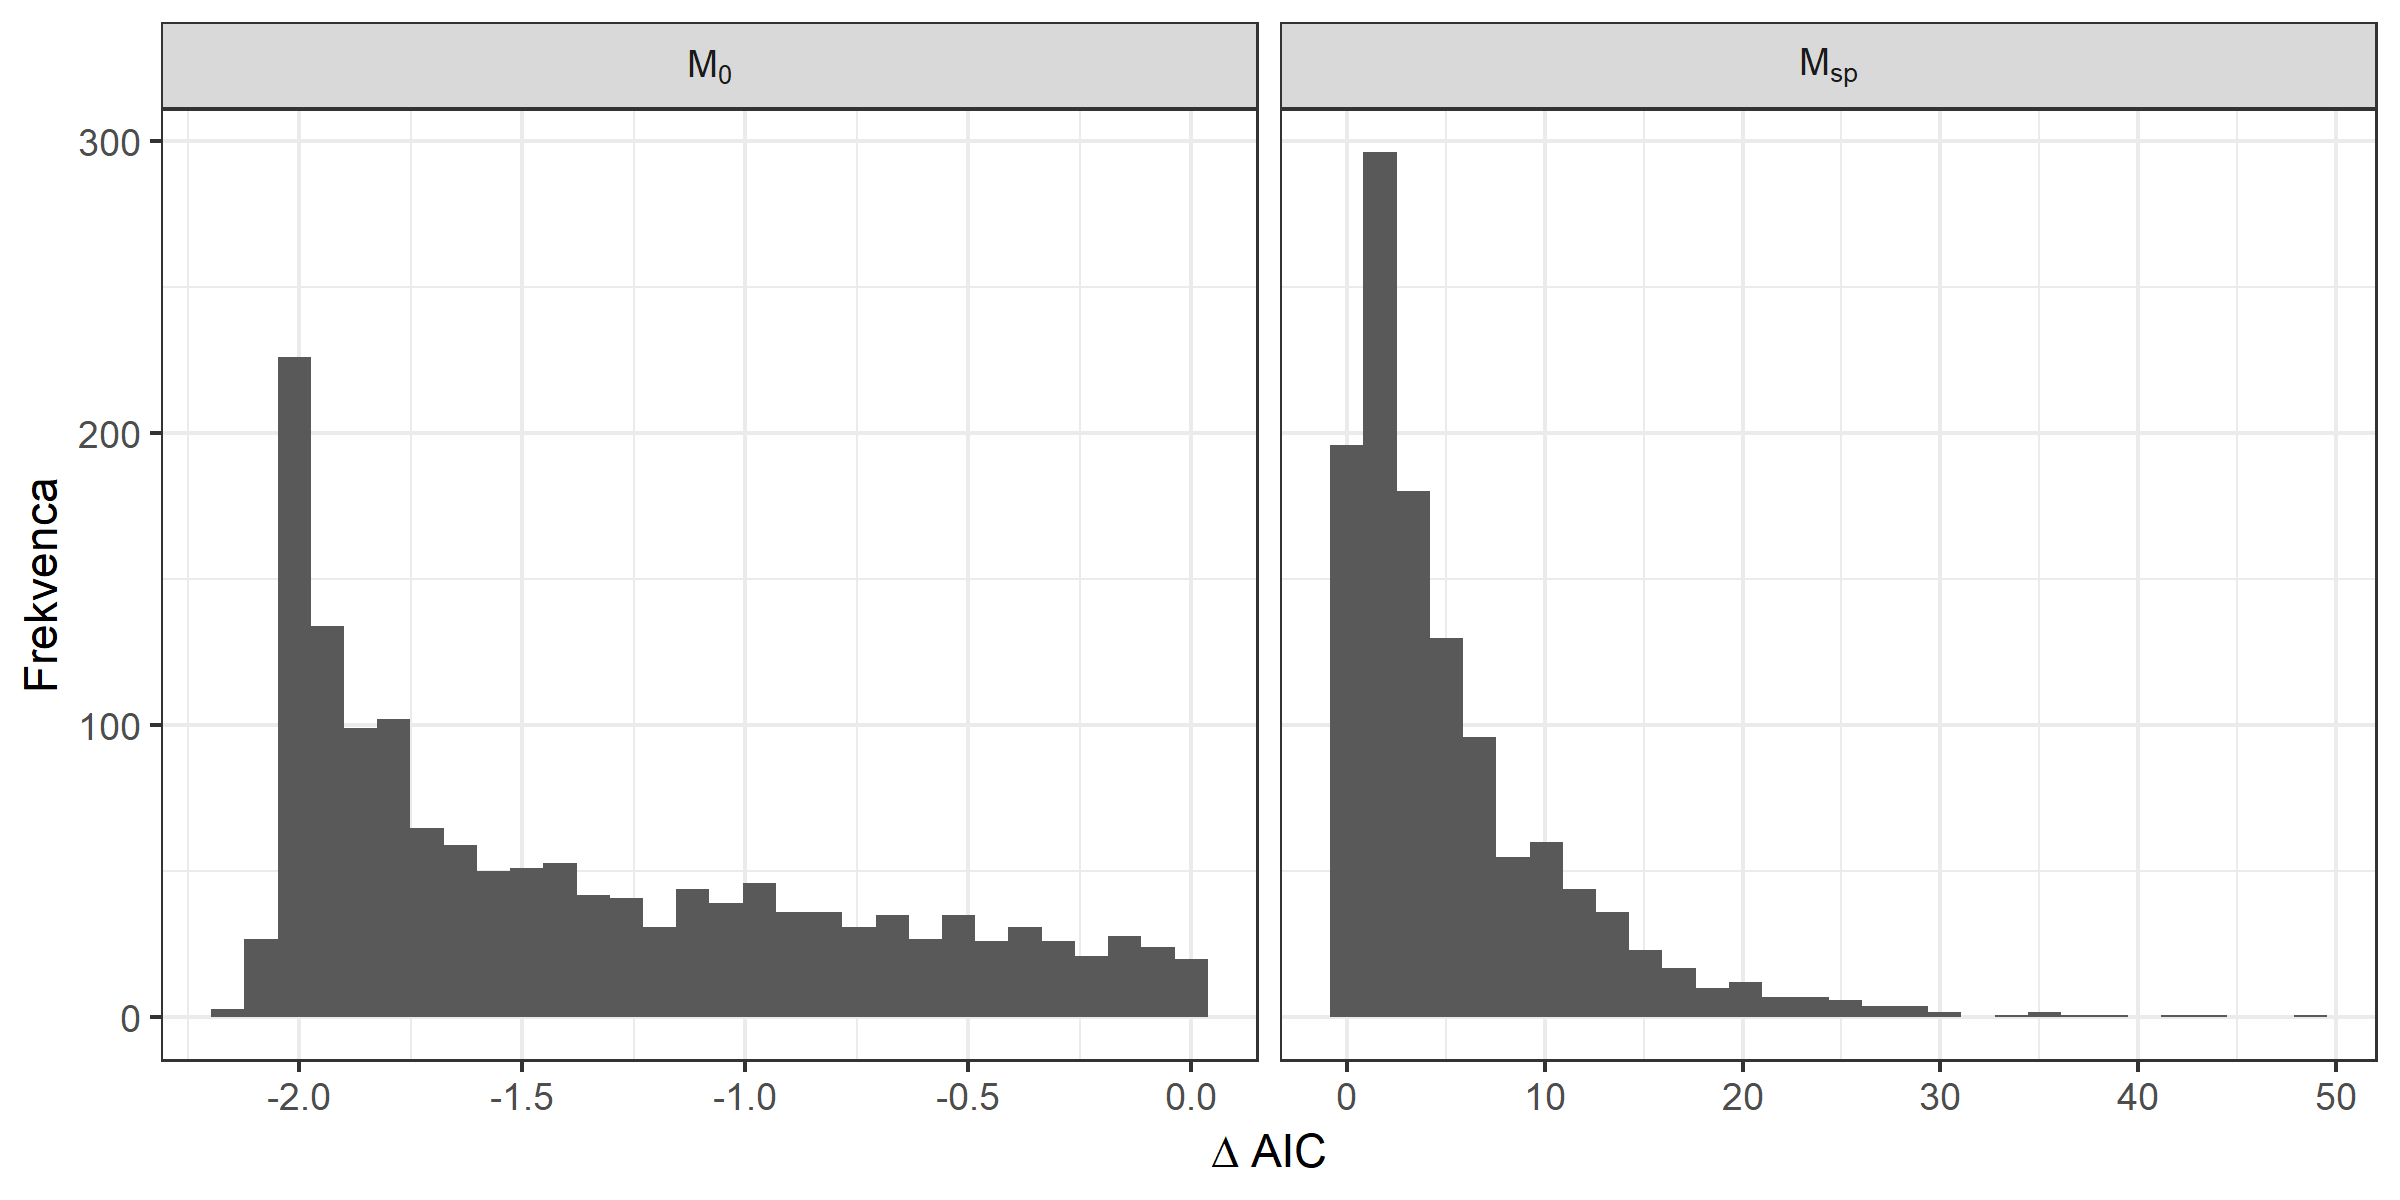
\includegraphics[width=1\linewidth]{C:/Users/romunov/Documents/workspace/doktorat/analiza/figures/E-8a_dAIC_glede_na_najboljsi_model.png}
    \label{sli:sub11.1}
  \end{subfigure}

  \begin{subfigure}[b]{1\textwidth}
    \centering
    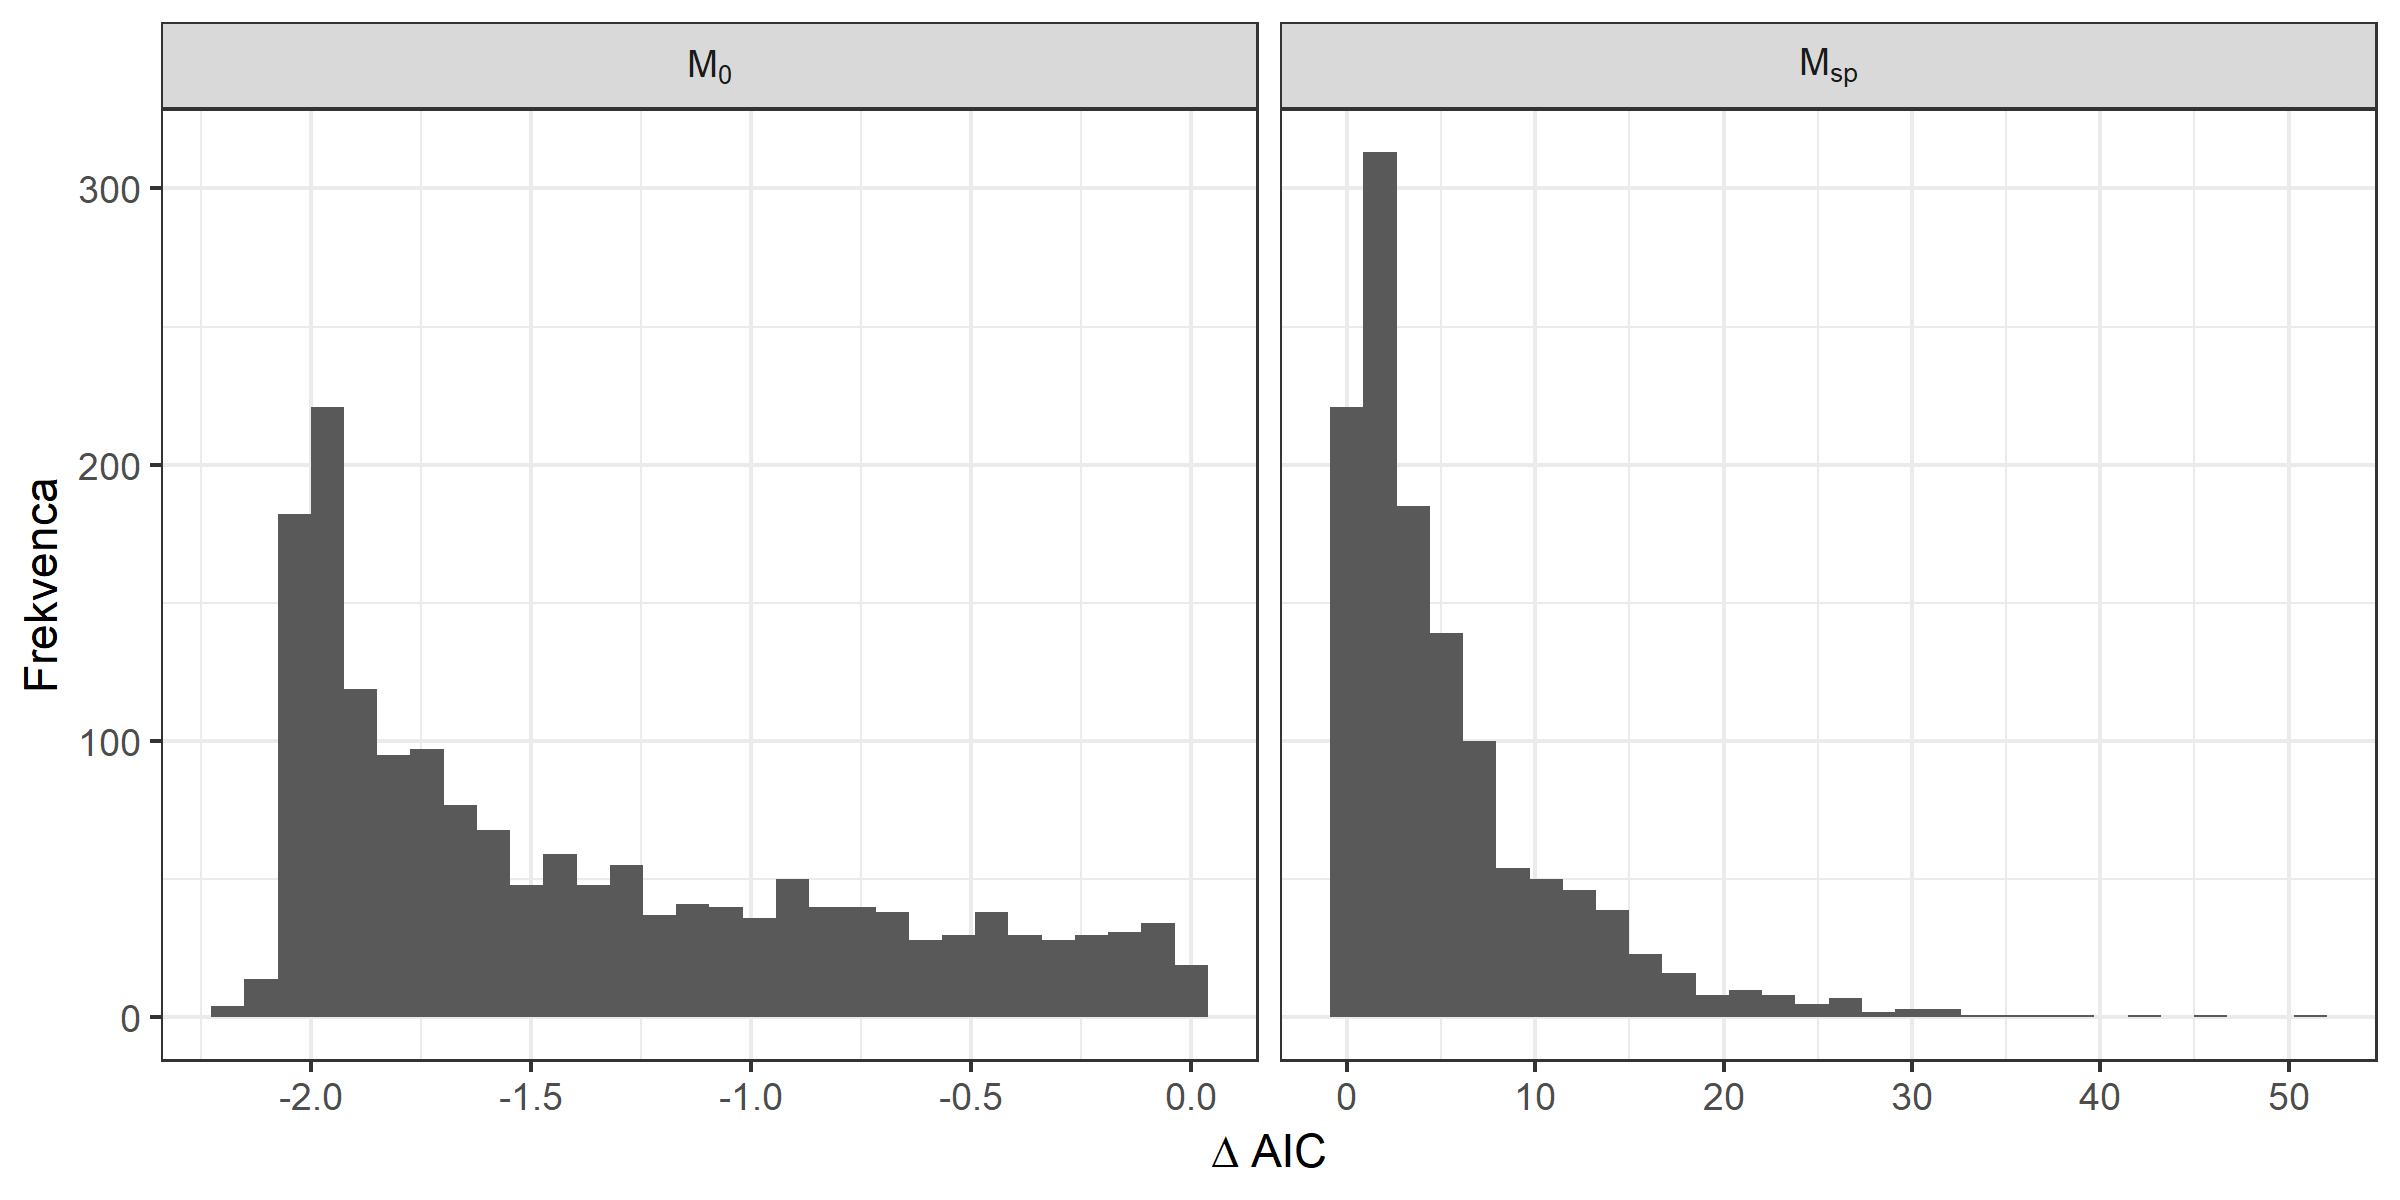
\includegraphics[width=1\linewidth]{C:/Users/romunov/Documents/workspace/doktorat/analiza/figures/N-8a_dAIC_glede_na_najboljsi_model.png}
    \label{sli:sub11.2}
  \end{subfigure}
  \caption[Podrobnejši prikaz porazdelitev razlik v AICc za modela $M_0$ in $M_{sp}$]{Podrobnejši prikaz porazdelitev razlik v AICc za modela $M_0$ in $M_{sp}$ s slike \ref{sli:slika10}. Zgornja dva histograma predstavljata vrednosti, kjer smo za izračun individualne spremenljivke uporabili empirično porazdelitev, spodnja pa vrednosti, kjer smo uporabili normalno porazdelitev. Previdni moramo biti pri razlaganju osi $x$, saj med modeloma nista neposredno primerljivi.

  \medskip

  Figure \ref{sli:slika11}: Detailed view of distribution of $\delta$AICc for models $M_0$ and $M_{sp}$ from figure \ref{sli:slika10}. Two histograms at the top and bottom represent simulations where individual covariate has been calculated using empirical and two-dimensional normal distributions, respectively. Note that $x$ axes are not directly comparable between graphs.}
  \label{sli:slika11}
\end{figure}
